% LaTeX mintafájl szakdolgozat és diplomamunkáknak az
% SZTE Informatikai Tanszekcsoportja által megkövetelt
% formai követelményeinek megvalósításához
% Modositva: 2011.04.28 Nemeth L. Zoltan
% A fájl használatához szükséges a magyar.ldf 2005/05/12 v1.5-ös vagy későbbi verziója
% ez letölthető a http://www.math.bme.hu/latex/ weblapról, a magyar nyelvű szedéshez
% Hasznos információk, linekek, LaTeX leirasok a www.latex.lap.hu weboldalon vannak.
%


\documentclass[12pt]{report}

%Magyar nyelvi támogatás (Babel 3.7 vagy későbbi kell!)
\def\magyarOptions{defaults=hu-min}
\usepackage[magyar]{babel}

%Az ékezetes betűk használatához:
\usepackage[utf8]{inputenc}
\usepackage{tgtermes} % betű tipus {times} nem kezeli jól az ő ű -t
\usepackage[T1]{fontenc}
\input glyphtounicode
\pdfgentounicode=1

%Az AMS csomagjai
\usepackage{amsmath}
\usepackage{amssymb}
\usepackage{amsthm}

%A fejléc láblécek kialakításához:
\usepackage{fancyhdr}

%Természetesen további csomagok is használhatók,
%például ábrák beillesztéséhez a graphix és a psfrag,
%ha nincs rájuk szükség természetesen kihagyhatók.
\usepackage{graphicx}
\usepackage{psfrag}

\usepackage{forloop}

\usepackage[usenames,dvipsnames]{xcolor}
\usepackage[draft]{pgf}
\usepackage{setspace}
\usepackage{todonotes}
\usepackage{pgf, tikz}

\usepackage{scrbase}
\usepackage{listings}
\newcaptionname{magyar}{\lstlistingname}{Kódrészlet}
\lstset{language=sql,
	keywordstyle=\color{BlueGreen},
	stringstyle=\color{BrickRed},
	commentstyle=\color{OliveGreen},
	morecomment=[l][\color{OliveGreen}]{\#},
	breaklines=true, postbreak=\raisebox{0ex}[0ex][0ex]{\ensuremath{\color{red}\hookrightarrow\space}}
}

\usetikzlibrary{arrows, automata}

%Tételszerű környezetek definiálhatók, ezek most fejezetenkent egyutt szamozodnak, pl.
\newtheorem{tét}{Tétel}[chapter]
\newtheorem{defi}[tét]{Definíció}
\newtheorem{lemma}[tét]{Lemma}
\newtheorem{áll}[tét]{Állítás}
\newtheorem{köv}[tét]{Következmény}

%Ha a megjegyzések és a példak szövegét nem akarjuk dőlten szedni, akkor
%az alábbi parancs után kell őket definiální:
\theoremstyle{definition}
\newtheorem{megj}[tét]{Megjegyzés}
\newtheorem{pld}[tét]{Példa}

%Margók:
\hoffset -1in
\voffset -1in
\oddsidemargin 35mm
\textwidth 150mm
\topmargin 15mm
\headheight 10mm
\headsep 5mm
\textheight 237mm

%Hyperlinkek:
\usepackage{hyperref}
\hypersetup{unicode=true}


\begin{document}
	
	%A FEJEZETEK KEZDŐOLDALAINAK FEJ ES LÁBLÉCE:
	%a plain oldalstílust kell átdefiniálni, hogy ott ne legyen fejléc:
	\fancypagestyle{plain}{%
		%ez mindent töröl:
		\fancyhf{}
		% a láblécbe jobboldalra kerüljön az oldalszám:
		\fancyfoot[R]{\thepage}
		%elválasztó vonal sem kell:
		\renewcommand{\headrulewidth}{0pt}
	}
	
	%A TÖBBI OLDAL FEJ ÉS LÁBLÉCE:
	\pagestyle{fancy}
	\fancyhf{}
	\fancyhead[L]{Minőségkinyerés borkóstolási adatokból, web és android alkalmazás fejlesztés}
	\fancyfoot[R]{\thepage}
	
	
	%A címoldalra se fej- se lábléc nem kell:
	\thispagestyle{empty}
	
	\begin{center}
		\vspace*{1cm}
		{\Large\bf Szegedi Tudományegyetem}
		
		\vspace{0.5cm}
		
		{\Large\bf Informatikai Tanszékcsoport}
		
		\vspace*{3.8cm}
		
		
		{\LARGE\bf Minőségkinyerés borkóstolási adatokból, web és android alkalmazás fejlesztés}
		
		
		\vspace*{3.6cm}
		
		{\Large Szakdolgozat}
		% vagy {\Large Szakdolgozat}
		
		\vspace*{4cm}
		
		%Értelemszerűen megváltoztatandó:
		{\large
			\begin{tabular}{c@{\hspace{4cm}}c}
				\emph{Készítette:}     &\emph{Témavezető:}\\
				\bf{Varga Tamás}  &\bf{Dr. Csendes Tibor}\\
				Programtervező Informatikus     &tanszékvezető egyetemi tanár\\
				hallgató&
			\end{tabular}
		}
		
		\vspace*{2.3cm}
		
		{\Large
			Szeged
			\\
			\vspace{2mm}
			2015
		}
	\end{center}
		
	\onehalfspacing
	%A \chapter* parancs nem ad a fejezetnek sorszámot
	\chapter*{Feladatkiírás}
	%A tartalomjegyzékben mégis szerepeltetni kell, mint szakasz(section) szerepeljen:
	\addcontentsline{toc}{section}{Feladatkiírás}
	A hallgató feladata egy olyan web és hozzá tartozó android alkalmazás készítése, amely képes borkóstolás során gyűjtött bor értékelések alapján több különböző algoritmus használatával a kóstolók rangsorolására. Az algoritmusok közül egyet a hallgatónak kell implementálnia. A web és android alkalmazásoknak képeseknek kell lenniük egymás közötti szinkronizációra, több felhasználó kezelésére, valamint a bevitt adatok és az alkalmazás állapotainak tárolására. Az android alkalmazásnak részben internet kapcsolat nélküli módban is használhatónak kell lennie.
	
	\chapter*{Tartalmi összefoglaló}
	\addcontentsline{toc}{section}{Tartalmi összefoglaló}
	
	\paragraph{A téma megnevezése}
	Minőségkinyerés borkóstolási adatokból, web és android alkalmazás fejlesztés.
	
	\paragraph{A feladat megfogalmazása}
	Web és android alkalmazás fejlesztése, amely képes bor értékelések alapján már létező algoritmusok által rangsorolni a borkóstolókat. A mobil alkalmazás felhasználó barát megvalósítása, amely bármilyen körülmény mellet valós idejű adatbevitelt is garantál.
	
	\paragraph{A megoldási mód}
	A web alkalmazás a következő címekről érhető el:
	\begin{itemize}
		\item \url{http://bor.tvarga.hu}
		\item \url{http://olga.inf.u-szeged.hu/borkostolas/} csak a Szegedi Tudományegyetem belső hálózatából.
	\end{itemize}
	
	Az android alkalmazás letölthető bármelyik fent említett URL -ről a jobb oldali floating menün keresztül, vagy az alábbi közvetlen linken: \href{http://bor.tvarga.hu/borkostolas.apk}{borkostolas.apk}
		
	\paragraph{Alkalmazott eszközök, módszerek}
	\begin{itemize}
		\item Web alkalmazás: 
		\subitem Programozási nyelvek: PHP, JavaScript, SQL
		\subitem Fejlesztői környezetek: SublimeText, PhpStorm
		\item Android alkalmazás:
		\subitem Programozási nyelvek: Java
		\subitem Fejlesztői környezetek: Android Studio
		\item Verziókezelés: GitHub
	\end{itemize}
	
	\paragraph{Kulcsszavak}
	Android, PHP, JavaScript, Borkóstolás
	
	%A tartalomjegyzék:
	\tableofcontents
	
	\chapter*{Bevezetés}
	\addcontentsline{toc}{section}{Bevezetés}
	
	Borkóstolók rangsorolásával, illetve minőségkinyeréssel, valamint borversenyek lebonyolításával már előttem is többen foglalkoztak. Bár még van kutatni való ezen a területen, jól működő algoritmus már több is ismert ilyen jellegű feladatok megoldására. Ezért ennek a szakdolgozatnak nem is újabb algoritmusok kifejlesztése, vagy már meglévők továbbfejlesztése a fő célja. Mivel található több olyan web alkalmazás is, amely egy specifikus egyszerű algoritmust, vagy talán egy sokat tesztelt komplexebbet használ, mégsem létezik egy közismert, modern és felhasználóbarát alkalmazás, amely egy igényes felhasználói felületen keresztül bemutatná ezen algoritmusok működését, lehetővé téve, hogy nyomon kövessük akár saját laikus eredményeinket neves szakértőkhöz viszonyítva.
	
	Mivel a mai világban a mobil eszközök egyre nagyobb teret hódítanak, az is célom volt, hogy egy olyan mobil (android) alkalmazás társuljon a web alkalmazáshoz amely egy könnyen kezelhető intuitív felületen keresztül lehetővé tegye a rendszer használatát, bizonyos funkciókat még offline üzemmódban is elérhetővé téve, kielégítve napjaink átlagos felhasználóinak igényeit. 
	
	A dolgozat elején röviden bemutatom az alkalmazás által használt algoritmusokat. Majd rátérek a weboldal és a mögötte álló rendszerek felépítésére, a hozzájuk társuló fejlesztői környezetek és eszközök rövid ismertetésére. Ezt majd a mobil (android) alkalmazás bemutatása követ, amelynél szintén kitérek a rendszer felépítésére, illetve a megvalósítást lehetővé tevő eszközökre,  erőforrásokra. Logikusan ezt a két alkalmazási felület (web és mobil) összefűzésének megvalósítása követi. Az összefoglalás előtt néhány teszten keresztül bemutatom a rendszer megbízhatóságát. Legvégül pedig bemutatok néhány olyan dolgot, amely segítette a munkámat, mint például verziókezelő rendszerek használata.
	
	\chapter{Borkóstoló algoritmusok}
	
	Ezen szakdolgozat keretében a CoHITS algoritmus került implementálásra, amely mellé csatlakozott néhány Borkóstolás projekt \cite{Borkostolas projekt} keretében használt már Szilárd Iván által implementált algoritmus, mint a Hamming, Koszinusz, Precedencia, Összefüggőségi. Ezeknél az algoritmusoknál a PageRank egy hasonlósági mátrixon propagál, ennek elemeit a borkóstolók páronkénti értékeléseinek inverz távolságából kapjuk, a hozzájuk illő távolság mértékek alkalmazásával (Hamming távolság, koszinusz távolság, precedencia távolság, összefüggősségi távolság) \cite{Borkostolas projekt}.
	
	\section{CoHITS}
	A CoHITS algoritmus a PageRank és a HITS algoritmuson egy kiterjesztett változata \cite{CoHITS}. A PageRank algoritmust Sergey Brin és Larry Page fejlesztette ki a Google kereső használatához \cite{PageRank} keresési találatok fontossági rangsorolásnak meghatározása céljából. Tőlük függetlenül Jon Kleinberg egy hasonló koncepcióval állt elő amely ugyan ilyen jellegű feladatot látott el \cite{HITS}.
	
	Nézzük is akkor az algoritmus borkóstolásra való alkalmazását. Legyen $ X $ és $ Y $ a kóstolók és borok. Ugyan abból a $p^0$ értékből indulunk ki minden $x_{i} \in X $ kóstolónál. Ekkor legyen $w'\left(\overrightarrow{x_{i}y_{j}}\right)$ az az értékelés amit $y_j$ bor kapott az $x_i$ kóstolótól és legyen $w\left(\overrightarrow{x_{i}y_{j}}\right)=w'\left(\overrightarrow{x_{i}y_{j}}\right)/\sum_{j \in Y}w'\left(\overrightarrow{x_{i}y_{j}}\right)$ a normalizáltja. Továbbá legyen $q_j^0$ érték (az $y_j$ borra) az értékelések átlaga. Majd definiáljuk a $w\left(\overleftarrow{x_iy_j}\right)$ az alábbi képen: tegyük fel, hogy $y_j$ bort $l$ különböző kóstoló kóstolta és legyen
	
	\begin{equation} \label{CoHITS sum of diff}
	D=\sum_{i \in X}|q_j^0-w'\left(\overrightarrow{x_iy_j}\right)|,
	\end{equation}
	
	az összegek különbsége az átlagtól az $y_j$ borra tekintve. Végül, legyen
	
	\begin{equation} \label{CoHITS transition probability}
	w\left(\overleftarrow{x_iy_j}\right)=\dfrac{|\sum_{i \in X}|q_j^0-w'\left(\overrightarrow{x_iy_j}\right)||}{\left(l-1\right)D}
	\end{equation} 
	
	Ekkor $\sum_{i \in X}w\left(\overleftarrow{x_iy_j}\right)=1$ tehát minden $w\left(\overleftarrow{x_iy_j}\right)$ súlyra lehet úgy tekinteni, mint egy átmeneti valószínűség $y_j$-ből $x_i$-be. Az \ref{CoHITS gráf} ábra a súlyok kiszámítására mutat egy konkrét példát.
	
	A két kóstoló közti súly $x_i$ és $x_j$ úgy definiálható, mint egy rejtett átmeneti valószínűség 1 által definiálva. Ekkor a $p=W_{xp}$ HITS egyenlet  $p=\left(p_1,p_2,...,p_m\right)$ megoldás megadja a kóstolók rangsorát.
	
	\begin{figure}[!ht]
		\begin{center}
			\begin{tikzpicture}[
			> = stealth, % arrow head style
			shorten > = 1pt, % don't touch arrow head to node
			auto,
			node distance = 4cm, % distance between nodes
			semithick % line style
			]
			
			\tikzstyle{every state}=[
			draw = black,
			thick,
			fill = white,
			minimum size = 22mm
			]
			
			\node[state] (taster1) {Kóstoló 1};
			\node[state] (wine2) [below of=taster1] {Bor 2};
			\node[state] (wine1) [left of=wine2] {Bor 1};
			\node[state] (wine3) [right of=wine2] {Bor 3};
			
			\path[->] (taster1) edge node {2/12} (wine1);
			\path[->] (taster1) edge node {3/12} (wine2);
			\path[->] (taster1) edge node {7/12} (wine3);
			
			\node[state] (taster1b) [below of=wine1] {Kóstoló 1};
			\node[state] (taster2) [below of=wine2] {Kóstoló 2};
			\node[state] (taster3) [below of=wine3] {Kóstoló 3};
			\node[state] (wine1b) [below of=taster2] {Bor 1};
			
			\path[->] (wine1b) edge node {4/12} (taster1b);
			\path[->] (wine1b) edge node {5/12} (taster2);
			\path[->] (wine1b) edge node {3/12} (taster3);
			
			\end{tikzpicture}
		\end{center}
		\caption{\label{CoHITS gráf} A gráf súlyai amikor a Kóstoló 1 a 20, 30 és 70 értékeléseket adott a Bor 1, Bor 2 és Bor 3 borokra, valamint a Bor 1 a 20, 30 és 70 értékeléseket kapott a Kóstoló 1, Kóstoló 2 és Kóstoló 3 -tól.}
	\end{figure}
	
	Tehát látható, hogy az így előállított algoritmust alkalmazni lehet egy borkóstolási gráfra kóstolók rangsorolásának céljából az ő képességeik és szakmai hozzáértésük alapján. Általánosságban az figyelhető meg, hogy az így előálló rangsor jobban teljesít, mint más egyszerű statisztikai algoritmusok. Ki tudja szűrni a hozzá nem értő kóstolókat \cite{CoHITS}.
	
	\section{Hamming}
	A Hamming-távolságot \eqref{Hamming-távolság} többnyire vektorok, karaktersorozatok, valamint bitminták közötti eltérések kimutatására használják. A Hamming-távolság csak azt mondja meg, hogy hány helyen nem illeszkedik az egyik minta a másikra. Legyen $ S_{1} $ és $ S_{2} $ két azonos hosszú minta.
	
	\begin{equation} \label{Hamming-távolság}
	D_{Hamming}\left ( S_{1},S_{2} \right )=\sum_{p=0}^{|S_{1}|}S_{1}\left(p\right)\neq S_{2}\left(p\right)
	\end{equation}
	
	Ez a távolság nem lesz megfelelő mérték vizsgálathoz, mivel nem túl informatív.
	
	\section{Koszinusz}
	Legyen $ \pi^1 $ és $ \pi^2 $ két permutáció-vektor. Ekkor ezek koszinusz távolságát az \eqref{Koszinusz-távolság} képlet szerint számíthatjuk ki, ahol $ || \cdot || $ az euklideszi normát jelöli.
	
	\begin{equation} \label{Koszinusz-távolság}
	D_{cos}\left(\pi^1,\pi^2\right)=1-\dfrac{\pi^1\cdot\pi^2}{||\pi^1||\cdot||\pi^2||}
	\end{equation}
	
	\section{Precedencia}
	A precedencia távolság meghatározásához definiálnunk kell először a precedencia mátrix fogalmát. Egy $ \pi $, $ n $ hosszúságú permutáció precedencia mátrixa, egy olyan bináris elemekből álló $ n \times n $-es $ P $ mátrix, amelyben $ P_{\pi_{i}\pi_{j}}=1, i<j $ egyébként $P_{ij}=0$, azaz a permutáció elemeinek sorrendjét kódoljuk egy bináris mátrixszal. A precedencia távolságot két $\pi^1$ és $\pi^2$ permutáció között ($P_{1}$ és $P_{2}$ a nekik megfelelő precedencia mátrix) a precedencia mátrixuk egyező nem nulla elemeinek számából számíthatjuk ki \eqref{Precedencia-távolság} szerint.
	
	\begin{equation} \label{Precedencia-távolság}
	D_{prec}\left(\pi^1, \pi^2\right)=\dfrac{n\left(n-1\right)}{2}-\sum_{i=1}^{n}\sum_{j=1}^{n}P_{ij}^1P_{ij}^2
	\end{equation}
	
	\section{Összefüggőségi}
	Az összefüggősségi távolság a szomszédos elemek azonos előfordulásából számítható. Legyen a két permutációnk $\pi^1$ és $\pi^2$, $n$ hosszúságúak, és a szomszédos elemek azonos előfordulásának száma $n_{adj}$.
	
	Szemléletesen: Legyen $N_{\pi}$ a $\pi$ permutáció összefüggőségi mátrixa. Kezdetben minden eleme legyen $0$, majd a $\pi$ permutáció minden $i$ elemére az $N_{pi}\left(\pi_{i},\pi{i+1}\right)=1$. A $\pi^1$ és $\pi^2$ permutációra kiszámoljuk az $N_{\pi^1}$ és $N_{\pi^2}$ mátrixokat. $n_{adj}$ az $N_{\pi^1}$
	és$N_{\pi^2}$ mátrixban azonos cellában lévő $1$-esek száma. 
	
	Ekkor az összefüggősségi távolság \eqref{Összeföggőségi-távolság} szerint számítandó.
	\begin{equation} \label{Összeföggőségi-távolság}
	D_{adj}\left(\pi^1,\pi^2\right)=n-n_{adj}-1
	\end{equation}
	\cite{Borkostolas projekt}
	
	\chapter{A weboldal}
	
	A weboldal kialakításánál számomra fontos szempont volt, hogy az egy letisztult könnyen kezelhető felületet prezentáljon a felhasználók felé. Ennek érdekében már a kezdetektől folyton szem előtt tartottam, hogy a stilisztikai elemek hogyan viszonyulnak egymáshoz, illetve külön figyelmet fordítottam arra, hogy a CSS (\textbf{C}ascading \textbf{S}tyle \textbf{S}heets) konzisztens megjelenést biztosítson a web alkalmazás minden oldalán. Ez azért is jó döntés volt, mert így sokkal könnyebb volt kisebb finomításokat végezni, mintha a stilisztikai definíciók közvetlen a PHP fájlokban található HTML tagokban szerepeltek volna.
	
	A web alkalmazás alapvetően három részből épül fel:
	
	\begin{itemize}
		\item Statikus oldalak
		\item Dinamikus oldalak
		\item Az android alkalmazást ellátó szolgáltatások
	\end{itemize}
	
	Statikus oldalnak akkor nevezünk egy weblapot, ha annak a tartalma nem változik. Attól is független, hogy a látogató kicsoda, hanyadszor jelentkezik be vagy, hogy honnan jelentkezik be stb..., tehát a tartalom konzisztens minden egyes látogatás alkalmával. Ez a megközelítés főképp akkor előnyös ha valami olyan tartalmat akarunk nyújtani a felhasználóknak amin egyáltalán nem áll szándékunkban változtatni, vagy csak nagyon ritkán.
	
	Dinamikus oldalakról akkor beszélünk amikor valamilyen feltétel vagy beavatkozás közvetlenül befolyásolja azt, hogy a felhasználó által megtekintett tartalom pontosan micsoda is. Legtöbbször akkor használatos, ha egy adatbázis tartalmát akarjuk megjeleníteni, vagy olyan felületet hozunk létre amely interakciót tesz lehetővé a felhasználó és a web alkalmazás között. Rengeteg programozási nyelv létezik ennek a célnak az ellátására. Én a PHP-t és a JavaScript-et választottam.
	
	Az android alkalmazást szolgáltatásokkal ellátó rész fő feladata, hogy a szerveren található adatbázishoz elérést biztosítson, mivel android alkalmazások nem tudnak közvetlenül csatlakozni egy távoli adatbázishoz. Ezért kell ez a közbülső réteg amely kiszolgálja a mobil eszköz kéréseit, illetve olyan tartalmak elérését teszi lehetővé amelyek közvetlenül valamilyen limitációs okokból nem lennének elérhetőek. Sokszor ezeket egy böngészőből megnyitva nem látunk semmit, ez teljesen természetes, mivel itt a hangsúly nem azon van, hogy emberek számára értelmezhető/olvasható tartalmat biztosítsunk, hanem fő célunk a web és a mobil alkalmazás közötti kommunikációs csatorna megteremtése. Tehát egy olyan környezet ahol csak gépek beszélnek egymással.
	
	\section{Iterációk}
	
	Az oldal megalkotásához egy agilis iterációs dizájn megközelítést alkalmaztam, amelyben egy rövid kezdeti tervezés után elkezdtem a tényleges munkát ami abból állt, hogy implementáltam az adott feladatot, majd az így elkészült munkát tesztelve prezentáltam a megrendelőnek (konzulensnek). A következő lépés, a tesztek során előkerülő hibák megbeszélése és azok lehetséges javítása, valamint az alkalmazás új funkciókkal való bővítése volt. Ez az utolsó három lépés, tehát az implementálás, tesztelés és hibajavítás, valamint további funkciókkal való bővítés képezte az iterációs dizájn megközelítésem ciklikus magját. Az iterációk során felhasznált eszközökre és technológiák ismertetésére csak az iterációs mérföldkövek ismertetése után fogok kitérni. 
	
	\subsection{Első mérföldkő}Az első mérföldkő folyamán először megbeszéltem a megrendelővel, hogy milyen elvárásokkal rendelkezek, illetve vázoltam az általam tervezett munkamenetet. Továbbá kiválasztottam a fejlesztéshez szükséges fejlesztői környezeteket és a használatukhoz elengedhetetlen eszközöket előkészítettem a projekt munkában való felhasználáshoz. Ekkor történt meg a felhasználói felület megjelenési terveinek elkészítése. Webszerver, domain és adatbázis létrehozás, illetve telepítés. A kész oldalszerkezeti tervekkel \ref{fig:Wireframe} neki kezdtem a grafikus elemek vizualizációjának, valamint implementáltam az oldalszerkezet statikus elemeit mint: Menü rendszer, fejléc, alsó információs sáv, kapcsolatok és egyéb hír csatornák megjelenítésért felelős elemeket.
	
	\begin{figure}[h]
		\centering
		\includegraphics[width=0.7\linewidth]{Wireframe}
		\caption[Első oldalszerkezeti terv]{Első oldalszerkezeti terv \label{fig:Wireframe}}
	\end{figure}
	
	\subsection{Második mérföldkő}A második mérföldkő során került sor a megrendelőtől kapott dokumentumok és források feldolgozására, majd azok feltöltése a projektbe főként statikus HTML elemekként, továbbá végrehajtása a megrendelő által kért grafikus és szerkezeti változtatásokat mint: Alsó információs sáv átmozgatása és re-faktorizációja egy oldalsó lebegő mozgó elemmé ($floating\ sidebar$), menüpontok átnevezése, fejléc logó frissítése. \linebreak A $borkostolasEredmenyek$ oldal átdolgozása az alábbi módon: Táblázatok  kettéválasztása. Vízszintes görgető sáv hozzáadása a borok táblázat felső- és alsó részéhez, amelyek együtt mozognak egymással, így megoldva a táblázat nagyságából fakadó kezelhetőségi problémát. Az előre láthatólag bekövetkező grafikai felépítés esetleges módosítása megkönnyítésének érdekében több stílus elemet is újabb osztályokba rendeztem, tehát egy átfogóbb re-faktorizáció történt. Ez mint később kiderült a további stilisztikai elemek hozzáadását és stilizálását is megkönnyítette.
	
	\subsection{Harmadik mérföldkő}A harmadik mérföldkő fő feladata az azt megelőző konzultáció során átbeszélt $demo$ oldal elkészítése volt. Itt került sor a CoHITS algoritmus megismerése, a hozzá tartozó szakirodalom áttanulmányozására majd az algoritmus implementálásának megkezdésére a projektbe. Ezt követte a korreláció és átlagtól való átlagos eltérés számolásának implementálása, de mint később kiderült ezek az algoritmusok nem tűrték jól a hiányos bemeneti adatokat ezért végül az általuk generált kimenet nem került felhasználásra. A mérföldkő végére a CoHITS algoritmus implementálásának befejezése és tesztelése maradt. Ezen mérföldkő keretén belül ismerkedtem meg a Google grafikonkészítő API-val, majd azt felhasználtam a CoHITS algoritmus, korreláció és átlagtól való átlagos eltérés adatsorok reprezentációjához.
	
	\subsection{Negyedik mérföldkő}A negyedik mérföldkő során egy másik projektből\cite{Borkostolas projekt} származó algoritmusok és azok már kész implementálásának feldolgozása és megismerése volt a fő feladat. Át kellett tekinteni a kapott kódbázist abból a célból, hogy ezeket is, mint majd további opciókat integráljam a rendszerbe. Az említett algoritmusok: Hamming, Koszinusz, Precedencia, Összefüggőségi. De még mielőtt ebbe bele kezdtem, kísérleteztem egy kicsit egy új grafikonrajzoló API (Charts.js) használata amely könnyebben, stílusosabban és személyre szabhatóbban reprezentálja az adatokat. Miután megkaptam a fent említett már implementált algoritmusokat, elkezdtem azokat integrálni az én projektem kódbázisába. Sajnos ez nem ment teljesen gördülékenyen, szükség volt a kapott kódbázisból előkerülő implementációs és működési problémákkal kapcsolatos kérdések átgondolására valamit konzultálásra ezekkel kapcsolatban, majd a hibák javítása. A sikeres hibaelhárítás és javítások után jött az algoritmusok és demo oldal működésének tesztelése.
	
	\subsection{Ötödik mérföldkő}Az ötödik mérföldkő bebizonyította, hogy érdemes volt jól megtervezni és szétválasztani az egyes stilisztikai elemeket, mivel a megrendelő ismét a menü rendszer, valamint a fejléc kép ismételt átrendezését és szerkesztését kérte. Továbbá új teszt adatok használatát javasolta a $demo$ menüpontban, amelyek már a friss adatokat tükrözik. Implementálásra került egy visszaigazolást kérő felhasználói felület amely fő célja a beviteli mátrix véletlen felülírásának meggátolása volt. Később a bevitel metódus megváltoztatása miatt ennek a funkcionalitása elévült. A korrelációt számoló kód működéséből fakadó hiba ki lett javítva, így már nem állt meg a számolás, ha a kapott hiányos adatsoron nem lehetett egyszerűen korrelációt számolni. Valamint megtörtént a tesztelések során előkerült további hibák kijavítása is.
	
	\subsection{Hatodik mérföldkő}A hatodik mérföldkő vissza hozta a régi grafikonrajzoló API-t (Google charts API), valamint megtörtént a grafikonokat megjelenítő elemek stilizálásnak egységesítése. Fő ok a visszaváltásra az volt, hogy az értékeket mint címkéket megjeleníthetővé tegyük az oszlopok mellett. A borszakértők személyiségi jogainak védése érdekében, a nevük anonimizálásra került. A web alkalmazás új funkciókkal bővült: Regisztráció, belépés. Ezt követte a $demo$ oldal teljes átdolgozása, így már az hozzá kapcsolódik a felhasználói rendszerhez. Ebből fakadóan a $demo$ oldal már csak regisztráció, illetve bejelentkezés után használható. \uppercase{í}gy a felhasználók a neves borszakértők által kóstolt borokat saját maguk is tudják értékelni.
	
	\subsection{Hetedik mérföldkő}A hetedik és egyben utolsó mérföldkő nagy részét a mobil android alkalmazás elkészítése és tesztelése tette ki, de itt valósult meg az őt kiszolgáló web szolgáltatások implementálása, valamint egy alap adminisztrációs felület létrehozása. Legvégül pedig elvégeztem némely kód csinosítást és re-faktorizációt a célból, hogy a kódom könnyebben olvasható és általában véve jobb tetszést keltsen az emberben.
	
	\section{Adatbázis}
	Annak ellenére, hogy a weboldal legelső változata perzisztens adat tárolás nélkül üzemelt és az implementált algoritmus tesztelése részben -e nélkül zajlottak, nem jelenti azt, hogy a végső változatból ez kimaradt volna, vagy esetleg egy nem teljesen kidolgozott adat tároló hierarchiával rendelkezne. Pontosan az ellenkezője az igaz. Az adatbázis táblák létrehozása előtt jelentős időt fordítottam azok megtervezésére, szem előtt tartva azt, hogy a tervezett alkalmazásoknak milyen igényei lesznek. Az adatbázis relációs sémáját a \ref{fig:dbmodel} ábra ábrázolja. Fontos még megemlíteni, hogy az adatbázis összes táblája $utf8\_unicode\_ci$ alapértelmezett karakter kódolást alkalmaz, amely biztosítja, hogy többek közt a magyar nyelvi sajátos karakteri is megfelelően tárolódjanak.
	
	\begin{figure}[!ht]
		\centering
		\includegraphics[width=0.7\linewidth]{../../Borkostolas_weblap/dbmodel}
		\caption[Adatbázis modell]{Adatbázis modell \label{fig:dbmodel}}
	\end{figure}
	
	Az adatbázist kiszolgáló szervernek az Oracle által fejlesztett MySQL-t választottam. Ezt ismerem a legjobban, valamint az sem elhanyagolható, hogy nyílt forráskódú. Talán ezért is rengeteg web szolgáltató által nagyon kedvelt gyakran alkalmazott megoldás. 
	
	\subsection{scores tábla}
	
	Ahogy az értékeléseket tartalmazó $scores$ táblát létrehozó szkript  \ref{lst:scores create} kódrészlet is tükrözi, látható, hogy a táblában a felhasználók azonosítóját $user\_id$ tartalmazó oszlop és a borok azonosítóját $wine\_id$ tartalmazó oszlop is mint $FOREIGN\_KEY$ szerepel, amik természetesen a borokat $wines$ és a felhasználókat $users$ tartalmazó táblák megfelelő oszlopaira hivatkoznak. Ezek segítik az adatbázis konzisztenciájának megőrzését. Amikor egy felhasználó vagy bor törlésre kerül akkor az $ON\ DELETE\ CASCADE$ megkötés hatására az értékeléseket tartalmazó $scores$ táblából azok a sorok is törlődni fognak amik így már nem létező azonosítókra hivatkoznának. Itt talán még érdemes kitérni arra is, hogy takarékossági okokból az értékelések maximum nyolc számjegyből állhatnak, amiben a decimális pontosságot három tizedes jegyig engedélyezzük. 

 	
	\noindent\noindent\begin{minipage}{\linewidth}
		\begin{lstlisting}[language=sql,label={lst:scores create}, caption={Az értékeléseket tartalmazó ($scores$) táblát létrehozó parancs}]
CREATE TABLE IF NOT EXISTS `scores` (
`user_id` int(11) DEFAULT NULL COMMENT 'user''s id',
`wine_id` int(11) DEFAULT NULL COMMENT 'wines''s id',
`score` decimal(8,3) DEFAULT NULL COMMENT 'score given by the user_id user for the wine_id wine',
`timestamp` timestamp NOT NULL DEFAULT CURRENT_TIMESTAMP ON UPDATE CURRENT_TIMESTAMP,
FOREIGN KEY (`user_id`) REFERENCES users(`user_id`) ON DELETE CASCADE,
FOREIGN KEY (`wine_id`) REFERENCES wines(`wine_id`) ON DELETE CASCADE
) ENGINE=MyISAM DEFAULT CHARSET=utf8 COLLATE=utf8_unicode_ci COMMENT='score data';
		\end{lstlisting}
	\end{minipage}
	
	Valamint az is jól látható, hogy egy időbélyeg oszlopban $timestamp$ nyomon követjük majd az értékelések módosításának időpontját. Ez elengedhetetlen a web és android alkalmazás között való effektív szinkronizációhoz. Végül talán még érdemes arra kitérni, hogy amelyik mező milyen értéket vehet föl és mik azok alapértelmezett értékek. A $user\_id$ és a $wine\_id$ helyzetét már tisztáztuk. Nem maradt más mint az értékeléseket tartalmazó $score$ és a módosítások időbélyegét nyomon követő $timestamp$. A $score$ mező értéke akár $NULL$ is lehet, így lehetővé téve a felhasználók számára, ha esetleg meggondolták magukat akkor töröljék a már meglévő értékelésüket. Ez lényegében csak egy praktikus megoldás, mert így amikor az alkalmazás egyszerre több értékelés eredményét próbálja módosítani, akkor azt meg tudja tenni egy $UPDATE$ SQL paranccsal, nem kell ennek az esetnek a külön kezelésére egy $DELETE$ utasítást írni. Valóban így több hely foglalódik le az adatbázisban, de ne felejtsük el, hogy olyan borok értékeléséről beszélünk amiket az adott felhasználó egyszer már értékelt. Én valószínűbbnek tartom azt, hogy valaki a kitörölt bort később újra értékeli, mint azt, hogy soha többet nem tér vissza hozzá. A $timestamp$ mező alapértelmezett értéke a $CURRENT\_TIMESTAMP$ ami másodperc pontossággal tartalmazza az időt, az alábbi formátumban: $Y-m-d\ h:i:s$ ahol $Y$ az év $m$ a hónap $d$ a nap mindegyik numerikus, majd $h$ az óra $i$ a perc és $s$ a másodperc két karakteres formátumban. $NULL$ helyett pedig $0000-00-00 00:00:00$ fog szerepelni a mezőben.
	
	\subsection{wines tábla}
	
	A borokat tartalmazó $wines$ tábla egyáltalán nem bonyolult. A tábla indexelését a \linebreak$wine\_id$ segítségével történek amely minden egyes új bor hozzáadásánál automatikusan növekszik eggyel az $AUTO\_INCREMENT$ -nek köszönhetően. Az évjáratot \linebreak$wine\_year$ és az árat $wine\_price$ tartalmazó mezőkön kívül az összes többi megadása kötelező. Az évjárat egy, maximum négy jegyű egész szám lehet, míg az ára akár hatvannégy jegyű is lehet. Jelenleg a borok ára magyar Forintban értendő. Ezek a megkötések főképp a projekt fejlesztése alatt megismert borkóstolási versenyek és adatbázisok szerkezeti felépítése miatt lettek így meghatározva. A többi mező kötelező szöveggel való feltöltését az alábbi táblázat \ref{tbl:wines-content} határozza meg:
	
	\begin{table}[!ht]
		\begin{center}
			\begin{tabular}{| l | l |}
				\hline
				\textbf{Mező} & \textbf{Tartalom} \\ \hline
				wine\_name & A bor neve \\ \hline
				wine\_winery & A pincészet neve \\ \hline
				wine\_location & A bor származási helye \\ \hline
				wine\_composition & A bor összetétele \\ \hline
			\end{tabular}
		\end{center}
		\caption{A borokat leíró tábla kötelező mezőinek felépítése \label{tbl:wines-content}}
	\end{table}
	
	\subsection{users tábla}
	
	A felhasználókra vonatkozó adatokat nyomon követő tábla neve az adatbázisban $users$. A tábla elsőre talán túl bonyolultnak tűnhet, de minden mezőnek fontos feladata van, amelyek lehetővé teszik egy kedvelt felhasználó kezelő modul használatát \cite{php-login}. A borokat tároló $wines$ táblához hasonlóan itt is van egy azonosító, még pedig a $user\_id$ amely a tábla indexelését látja el és automatikusan növekszik eggyel az $AUTO\_INCREMENT$ -nek köszönhetően amikor egy új felhasználó regisztrál a rendszerbe. A $user\_id$ nem az egyetlen egyedi $UNIQUE$ azonosító a táblában, a felhasználó nevét tároló $user\_name$, valamint a regisztrált felhasználó által megadott e-mail címet tároló $user\_email$ mező is egyedi. Ezzel azt meggátolva, hogy valaki már egy létező e-mail címmel vagy felhasználó névvel újból regisztráljon. Ezek voltak a regisztráció során kötelezően megadandó mezők egy része. Később még szó lesz a jelszó kezelésről is. A regisztráció után már aktivált felhasználó státuszt a $user\_active$ követi nyom, úgy, hogy azokhoz akik még nem látogatták meg a regisztrációt visszaigazoló e-mailben kapott linket, hozzájuk nullát rendel, akik pedig ezt már megetették egyet kapnak, ez arra szolgál, hogy csak olyan e-mail címeket zároljon a rendszer amelyek már regisztráció után aktivált felhasználó fiókhoz tartoznak. A felhasználót azonosító süti kulcs a $user\_rememberme\_token$ mezőben tárolódik, amely két hétig érvényes, ezzel lehetővé téve a web alkalmazás számára, hogy felismerje az ismételt látogatókat még akkor is ha már más $HttpSession$ be tartoznak. A hibás bejelentkezések számát a $user\_failed\_logins$ mező tárolja. Többek között ennek pontos felhasználását később fogom részletezni a felhasználó kezelő rendszer részletes ismertetésénél. A regisztráció során használt IP cím a $user\_registration\_ip$ -ben tárolódik el. Adminisztrátori jogosultság megadását teszi lehetővé a $user\_permission$ mező, amelynek alapértelmezett értéke $0$, $1$ pedig az adminisztrátori jogosultságot szimbolizálja. A még nem tárgyalt mezőket két csoportra bonthatjuk, az egyik amely valamilyen hash stringet tartalmaznak mint a: 
	\begin{itemize}
		\item$user\_password\_hash$
		\item$user\_activation\_hash$
		\item$user\_password_reset\_hash$
	\end{itemize}
	A másik csoport pedig olyan mezők, amelyek valamilyen tevékenységet nyomon követő idő bélyeget tárolnak mint a: 
	\begin{itemize}
		\item$user\_password\_reset\_timestamp$
		\item$user\_last\_failed\_login$
		\item$user\_registration\_datetime$ 
	\end{itemize}
	Nézzük először az utóbbit, az idő bélyeg típust tároló mezőket. A \linebreak $user\_password\_reset\_timestamp$ arra szolgál, hogy nyomon tudjuk követni, hogy a felhasználó vagy esetleges támadó mikor igényelt jelszó újra beállító e-mailt. A \linebreak$user\_last\_failed\_login$ mező a legutolsó hibás bejelentkezés időpontját tárolja. A \linebreak$user\_registration\_datetime$ -ben tárolt időpontra pedig majd a regisztrációt visszaigazoló és aktiváló e-mail linkjének kezelésekor lesz szükség. Végül röviden azokról a mező típusokról amelyek valamilyen hash stringet tárolnak, mivel arra, hogy mi a hash és miért de főképp milyen módon van használva, majd többek között később térek ki a felhasználó kezelő rendszer részletes ismertetésénél. A $user\_password\_hash$ tárolja a felhasználó jelszavát hashelt formátumban. A regisztráció után küldött aktivációs e-mailhez használt aktivációs link validitásának ellenőrzésére szolgáló hasht a  $user\_activation\_hash$ tárolja. $user\_password\_reset\_hash$ pedig az új jelszót igénylő e-mail link hitelesítésére használt hasht tárolja.
	
	\section{CSS}
	CSS avagy \textbf{C}ascading \textbf{S}tyle \textbf{S}heets egy stilisztikai leíró nyelv amelynek célja, hogy leírja miképp formázódjanak és jelenjenek meg egy dokumentum elemei amelyeket egy markup nyelven írtak. Markup nyelvnek nevezzük az olyan nyelveket amelyek szintaktikailag megkülönböztethetőek a dokumentum szövegétől, jelen esetben ez a HTML, amely előre definiált prezentációs sémákkal rendelkezik, ami azt jelenti, hogy egy adott specifikáció adja meg, hogy az adatokat milyen módon jelenítse meg a rendszer. 
	
	A CSS-t először Hakon Wium Lie terjesztette elő 1994 Októbar 10. -én \cite{CSS-origin} a weblapok stílusát leíró nyelvként a W3C (World Wide Web Consortium, a világháló szabványaiért felelős nemzetközi szervezet) publikus levelezőlistáján. A CSS 1 specifikációja elkészültekor még nem volt olyan böngésző amely teljesen támogatta volna azt. Két évvel később a CSS 2 többek között bemutatta elemek abszolút, relatív és fixált pozicionálását, valamint bevezette a z tengely mentén való indexelés lehetőségét. A CSS 3 tól nem beszélhetünk W3C által elfogadott szabványról, ez a verzió főképp abban tér el elődjeitől, hogy egy moduláris felépítést követ. Minden modul kiterjeszti valamilyen módon, vagy új képességekkel látja el a korábbi CSS 2 -es funkciókat, ezzel megőrizve a visszafelé kompatibilitást. 
	
	Tagadhatatlan, hogy a CSS a webfejlesztés egyik fő sarokköve. Létrehozásának fő oka az volt, hogy a HTML oldalak tartalmi, illetve prezentációs része könnyen szétválasztható legyen. Ez a szeparáció azért is fontos, mert így nagyobb flexibilitást nyerhetünk a prezentáció területén, valamint lehetővé válik a HTML oldalak formázottságának megosztása egy egységes CSS fájlnak köszönhetően. Ezzel csökken a tartalmi oldalak komplexitása, valamint kevesebb lesz bennük az ismétlődés. Előnyök között mindenképpen említésre méltó, hogy így könnyebben lehetséges ugyan azt a markup nyelv által leírt dokumentumot több különböző stílusban megjeleníteni attól függően, hogy kinek, illetve milyen célra szánt az adott tartalom. Pontosabban ez alatt azt értjük, hogy a megjelenítés különböző lehet akár egy képernyőn, nyomtatásban, hangosan (képernyő felolvasáskor) vagy Braille billentyűs eszközökön. Továbbá az is lehetséges, hogy a megjelenítendő tartalmat illeszkedjen az adott eszköz képernyő méretéhez.
	
	Számomra, mint már korábban említettem a CSS fő előnye az volt, hogy a web alkalmazás stilisztikai felépítést egy fájlból könnyedén tudtam módosítani. De sajnos nem csak előnye van a CSS használatának. Az ember könnyen bele tud futni néhány igen bosszantó limitációba, mint például elemek vertikális rendezése. Míg a vízszintes elrendezés általánosságban könnyen kezelhető, a vertikális sokszor nem túl intuitív módon valósítható csak meg, ha egyáltalán megvalósítható. Egyszerű feladatok mint például egy elem vertikálisan való középre zárása, vagy a lábléc limitálása, hogy ne legyen magasabb mint a viewport alja, vagy nem intuitív komplikált szabályrendszert igényel, vagy olyan szabályokat igényel, amelyek nem túl bonyolultak, viszont kevéssé támogatottak. Kétségtelen, hogy használatának előnyei túlnyomó részben vannak hátrányaihoz képest. Némelyikbe azért konkrétan én is bele futottam és jelentős kísérletezgetésbe telt mire sikerült olyan szabályrendszert alkotni a leíró nyelvben amely a számomra elfogadható megjelenítést tette lehetővé. A kulcs az volt, hogy minden fő elemet egy konténerbe kellett tegyek amelyek egy $clear:both;$ tulajdonsággal rendelkeznek, majd ezeken belül már könnyebben tudtam pozicionálni a további elemeket. Ennek megértéséhez azt kell tudni, hogy a CSS -ben három fő pozicionálási mód van. 
	
	\paragraph{Normal flow}Az $inline$ elemek úgy vannak elrendezve, mint a betűk egy szavakat tartalmazó szövegben, tehát egymás után a rendelkezésre álló területen amíg van szabad hely, ha elfogy a hely, akkor egy új sorban folytatódnak. $Block$ elemek vertikálisan rakhatók össze, mint a paragrafusok vagy mint a felsorolások egyes pontjai. A $normal flow$ lehetővé teszi $inline$ elemek vagy $blokkok$ relatív pozicionálását.
	
	\paragraph{Flaot} Egy lebegő elem kikerül a $normal\ flow$-ból és balra vagy jobbra igazodik amennyire csak lehet a rendelkezésre álló szabad területen. A többi tartalom majd ennek az oldalán lebeg.
	
	\paragraph{Absolute positioning}Egy abszolút módon elhelyezett elem nem foglal helyet és nincs hatással a $normal flow$ típusú elemekre. Egy maghatározott saját területet foglal el a konténerében a többi elemtől függetlenül.
	
	\paragraph{Position}Nem meglepő módon négy pozíció van: $top$ - fel, $bottom$ - le, $left$ - balra, $right$ - jobbra. Ugyan csak négy lehetséges értéke lehet a $positio$ tulajdonságnak. Amennyiben egy elem $static$ -tól eltérő módon van elhelyezve, akkor a további tulajdonságok $top$, $bottom$, $left$, $right$ eltolás, illetve pozíció definiálásra szolgálnak. A négy lehetséges érték:
	
	\begin{enumerate}
		\item\textbf{Static}: Az alapértelmezett érték amely a $normal\ flow$ -ba teszi
		\item\textbf{Relative}: Az elem a $normal\ flow$ -ba kerül majd abból a pozícióból eltolódik. A további elemel úgy kerülnek elrendezésre mintha az eredeti elem ott maradt volna.
		\item\textbf{Absolute}: Abszolút pozicionálást definiál. Az eleme a legközelebb nem $static$ elemű őséhez képest lesz pozicionálva.
		\item\textbf{Fixed}: Az elem abszolút pozicionálásra kerül egy fixált pozícióban a képernyőn még akkor is ha az egész dokumentum el van görgetve.
	\end{enumerate}
	
	\paragraph{Float és clear}A $float$ tulajdonságnak három különböző értéke lehet. Abszolút vagy fixen pozicionált elemek nem lehetnek $float$ típusúak. Más elemek normálisan lebegnek a többi $float$ típusú elem körül, hacsak azt az $clear$ tulajdonságuk meg nem gátolja.
	\begin{enumerate}
		\item\textbf{left}: Az elem annak a vonalnak a bal oldalán jelenik meg ahol eredetileg jelent volna meg, a többi elem a jobb oldalán lesz.
		\item\textbf{right}: Az elem annak a vonalnak a jobb oldalán jelenik meg ahol eredetileg jelent volna meg, a többi elem a bal oldalán lesz.
		\item\textbf{clear}: Arra kényszerít egy elemet, hogy az $clear$ által meghatározott elem bal oldalán legyen $clear:left$ vagy jobb oldalán $claer:right$ vagy esetleg mindkét oldalán $clear:both$.
	\end{enumerate}
	
	Kellő kísérletezés és gyakorlás után azért elérhető egy olyan struktúra amely ezeket megfelelően egymásba ágyazva a kívánt kinézetet nyújtja. 
	
	Érdemes még azért a CSS szintaktikájával is tisztában lenni. Röviden egy CSS szabály egy $selector$-ból és egy deklarációs blokkból épül fel.
	
	\noindent\begin{minipage}{\linewidth}
		\begin{lstlisting}[language=html,label={lst:css syntax}, caption={CSS szintaxis}]
h2 {color: #bb1f42; font-size: 1.2em;}
		\end{lstlisting}
	\end{minipage}
	
	Konkrétan a \ref{lst:css syntax} kódrészletben látott CSS kódnál a $h2$ a $selector$ őt követi a deklarációs blokk amely két deklarációt tartalmaz. Egy deklarációnak két része van, egy a tulajdonságot megnevező része, ez van a $:$ előtt, és egy azt követő rész amely az értéket tartalmazza. Lehetséges még több $selector$ összecsoportosítsa, amelynek köszönhetően jócskán csökkenthető az ismétlődő kód. Ugyan ezt segíti elő az is, hogy a CSS alapvetően támogat öröklődést, így egy felső konténeren definiált tulajdonság mindig lefelé a gyermekei felé propagál. Természetes a kevesebb kódnak más jó mellékhatása is van, mint a gyorsabban töltődő weboldal és kisebb sávszélesség használat. A $selector$ több típusú is lehet és ezeket kombinálni is lehet. A \ref{lst:css syntax} kódrészletben látottat $element selector$ -nak hívják, amely egy adott típusú elemet választ ki. A $class selector$ az olyan elemekre fog vonatkozni amik az adott $class$ attribútummal rendelkeznek. Ilyenkor egy pontot teszünk a $selector$ elé. Némely elem rendelkezhet különböző típusokkal is, pl.: egy $checkbox$ típusú $input$ elemre a $selector$ az alábbi módon nézne ki: $input[type=checkbox]$.
	
	\section{PHP}
	A PHP ($PHP:\ Hypertext\ Preprocessor$) egy széles körben elterjedt nyílt forráskódú általános célokra kifejlesztett szkript nyelv amely különösképpen alkalmas webes fejlesztésre, valamint HTML -be ágyazható. Ezt az alábbi példa \ref{lst:php hello world} kódrészlet szemlélteti.
	\noindent\begin{minipage}{\linewidth}
		\begin{lstlisting}[language=html,label={lst:php hello world}, caption={PHP Hello World!}]
<!DOCTYPE HTML PUBLIC "-//W3C//DTD HTML 4.01 Transitional//EN"
"http://www.w3.org/TR/html4/loose.dtd">
<html>
<head>
  <title>Pelda</title>
</head>
<body>
  <?php
  echo "Hello Vilag!";
  ?>
</body>
</html>
		\end{lstlisting}
	\end{minipage}
	A PHP kód egy különleges nyitó és záró $<?php\ ?>$ struktúrában helyezkedik el, ezzel lehetővé téve, hogy ki és be lépjünk a PHP-ba. A PHP-t azt különbözteti meg a kliens oldali szkriptektől, mint például a JavaScript, hogy a kód a szerver oldalon hajtódik végre, itt generálódik a HTML tartalom amelyet majd a webszerver küld a kliensnek. Az is megoldható, hogy egy webszervert úgy konfiguráljunk, hogy az a PHP-t tartalmazó HTML fájlokat is dolgozza fel. Ekkor a felhasználó nem fogja megtudni, hogy mi neki most éppen egy PHP által generált tartalmat mutatunk.
	
	Annak ellenére, hogy a PHP egy szkript nyelv robusztus alkalmazások létrehozására is használható, erre kiváló példa többek között a Facebook vagy akár a Wikipedia. Személy szerint ez előtt nem sokat foglalkoztam a PHP -val csak kisebb weboldalak létrehozására használtam, nem igazán követtem nyomon a nyelv fejlődését amely eredetileg a PHP/FI névvel lett létrehozva 1994 -ben Rasmus Lerdorf által. Ez az első változat egy egyszerű Common Gateway Interface (CGI) bináris állomány volt a C programozási nyelven írva amelynek fő feladata az ő személyes honlapjának egy eszköze volt. Ez már nagyon régen volt és a nyelv rengeteg változtatáson és javításon esett át. Most már a PHP 5. verziójánál tartunk. Én is ezt a verziót használtam, amely 2004 -ben lett kiadva. Fő vezérlő magja a $Zend\ Engine\ 2.0$ amely egy tucatnyi új szolgáltatás között egy új objektum modellt is tartalmaz. Jelenleg több tucatnyi fejlesztő dolgozik a PHP továbbfejlesztésével, amely továbbá pár tucat másik fejlesztőnek ad munkát akinek a feladata a PHP -hez kapcsolódó támogató projektek fejlesztése és dokumentálása. Ez csak egy korábbi éveken alapuló becslés, de nyugodtan mondhatjuk, hogy a PHP több tíz vagy akár száz millió domain-re van telepítve világszerte \cite{php-history}.
	
	A PHP nyelv általános felépítésére és szintaxisára nem térek ki, egyrészt azért, mert már egy elég régi nyelv amelynek alapjai régóta ismertek, valamint azért is, mert elég közel a $C$ nyelvhez, amely még ismertebb. Viszont mindenképpen ejtenék pár szót a nyelv sajátosságáról, főkép arra fókuszálva, hogy hogyan történik az állapotkövetés, illetve adatbázis elérés.
	
	\subsection{PHP Data Objects (PDO)}
	A PHP Data Objects (PDO) a PHP adatbázis elérést nyújtó interfésze. Minden adatbázis meghajtó amely implementál egy PDO interfészt elérhetővé tehet az adott adatbázisra specifikus funkciókat. Természetesen önmagában a PDO alkalmatlan adatbázis kezelésre, mindenképpen egy konkrét adatbázis meghajtót kell használni. Mivel a web alkalmazást egy $MySQL$ adatbázis szerver szolgálja ki ezért én a hozzá tartozó $PDO\_MYSQL$-t használtam. A PDO alapértelmezetten együtt jár a PHP 5.1-el és elérhető PECL kiterjesztésként is PHP 5.0 alatt, de mivel a PDO -nak szüksége van PHP 5 magjában bemutatott objektum orientáltságra, ezért a PDO nem fut korábbi PHP verziókon. 
	
	\noindent\begin{minipage}{\linewidth}
		\begin{lstlisting}[language=php,label={lst:php pdo connection}, caption={PHP PDO Connector használata}]
private function databaseConnection(){
  if ($this->db_connection != null) {
    return true;
  } else {
    try {
      $this->db_connection = new PDO('mysql:host='. DB_HOST .';dbname='. DB_NAME . ';charset=utf8', DB_USER, DB_PASS);
      return true;
    } catch (PDOException $e) {
      $this->errors[] = MESSAGE_DATABASE_ERROR . $e->getMessage();
    }
  }
  return false;
}
		\end{lstlisting}
	\end{minipage}
	
	A \ref{lst:php pdo connection} kódrészlet a bejelentkeztető modul egyik metódusán keresztül mutatja be, hogy hogyan lehet a PHP PDO -vel adatbázis kapcsolatot létrehozni. Először is ellenőrzésre kerül, hogy létezik -e már felépített adatbázis kapcsolat, nyilván ha már igen, akkor nincs mit tenni, de ha még nem, akkor létrehozunk egy új PDO objektumot, úgy, hogy a konstruktorának átadjuk az adatbázis címét, nevét, azt a felhasználót amelyikkel csatlakozni szeretnénk és természetesen a hozzá tartozó jelszót. Ezek a kódrészletben sorra a $DB\_HOST$, $DB\_NAME$, $DB\_USER$ $DB\_PASS$ amelyek egy külön konfigurációs fájlban kerültek definiálásra. Itt fontos még megemlíteni, hogy az adatbázis nevének megadásakor egyben megadjuk a karakter kódolást is, mivel ennek elhanyagolása biztonsági problémákat okozhat \cite{PDO-charset-security}. Természetesen a kódunknak készen kell állni esetleges nem várt események bekövetkezésére, ezért mindez egy $try\ - catch$ blokkban zajlik le, a remélhetőleg nem fellépő hibaüzeneteket pedig egy az azok tárolására létrehozott tömbben tároljuk, amiből majd később könnyen kiolvashatók, ha esetleg értesíteni akarunk valakit róla.
	
	Az adatbázis kapcsolatot nagyon egyszerű bezárni ahogy a \ref{lst:php pdo close connection} kódrészlet is mutatja. Ez nagyon fontos is, hogy mindig bezárjuk miután befejeztük a használatát, mivel sok szolgáltató limitálja, hogy hány aktív kapcsolatot kezel az adatbázis szerverük.
	
	\noindent\begin{minipage}{\linewidth}
		\begin{lstlisting}[language=php,label={lst:php pdo close connection}, caption={PHP PDO kapcsolat lezárása}]
db_connection = null;
		\end{lstlisting}
	\end{minipage}
	
	Miután sikeresen létrehoztunk egy aktív adatbázis kapcsolatot SQL utasításokat a \ref{lst:php pdo sql query} kódrészletben látott módon indíthatunk. A példában éppen lekérjük egy felhasználó összes információját, majd az így kapott információkat egy objektumban adja vissza a $fetchObject\left(\right)$ metódus. Tehát például a $user\_id$ a \ref{lst:php pdo result handling} kódrészletben látottak szerint lesz elérhető. Használatos még többek között a $fetchAll\left(\right)$ ami az SQL lekérdezés által visszaadott összes sort egy-egy tömbben adja vissza. Hasznos lehet még ismerni a $rowCount\left(\right)$ metódust, ami megadja az SQL parancs által érintett sorok számát.
	
	\noindent\begin{minipage}{\linewidth}
		\begin{lstlisting}[language=php,label={lst:php pdo result handling}, caption={PHP PDO eredmény kezelés}]
$user_id = $result_row->user_id;
		\end{lstlisting}
	\end{minipage}
	
	Vegyük észre, hogy az SQL lekérdezésbe nem konkatenáljuk bele a változókat, ha ilyesmit tennénk, akkor az alkalmazásunkat nagyon könnyen feltörhetnék, hiszen éppen ilyen programozói hibákat kihasználva működnek az $sql injection$ jellegű támadások. Tehát, ha változókat akarunk használni az SQL lekérdezésünkben, akkor a $prepare\left(\right)$ metódusban a behelyettesítendő helyre kettősponttal megelőzött változónevet kell írni, amelyet majd a $bindValue\left(\right)$ metódussal fogunk ténylegesen a mi változónkhoz kötni. Ez első paraméterként egy stringet vár, ami az SQL lekérdezésben szereplő változó helyét határozza meg. A második paramétere a mi PHP változónk, aminek az értékét az SQL parancsban szeretnénk használni. A harmadik és egyben utolsó na meg opcionális paraméter pedig az első paraméterre vonatkozóan definiálja annak adat típusát. Az $execute\left(\right)$ -hez nem kell sokat hozzáfűzni, egyszerűen végrehajtja a fentiek szerint előkészített SQL parancsot.
	
	\noindent\begin{minipage}{\linewidth}
		\begin{lstlisting}[language=php,label={lst:php pdo sql query}, caption={PHP PDO SQL lekérdezés}]
$query_user = $this->db_connection->prepare('SELECT * FROM users WHERE user_name = :user_name');
$query_user->bindValue(':user_name', $user_name, PDO::PARAM_STR);
$query_user->execute();
$result_row = $query_user->fetchObject();
		\end{lstlisting}
	\end{minipage}
	
	\subsection{Állapotkezelés és követés}
	Állapotkezelésre, illetve nyomkövetésre minden kicsit is bonyolultabb felhasználókat kezelő alkalmazásnak szüksége van. Mivel a HTTP egy állapot nélküli protokoll ezért amikor egy web szerver végrehajtotta egy kliens kérését a kapcsolat a kettő között megszakad. Tehát, más szóval, a szerver nem tudja felismerni, hogy egy kérés sorozat ugyan attól a klienstől származik, viszont ez egy nagyon fontos dolog főképp akkor, amikor különböző oldalak között navigálunk a web alkalmazásunkban. Ennek a problémának az orvosolására többféle megoldás is létezik. Konkrétan en a PHP nyelveben az állapotkezelésnek négy főbb fajtáját használtam. 
	
	Sütik avagy $cookies$ alapvetően olyan stringek amik több mezőt is tartalmazhatnak. A válasz fejlécében a szerver egy vagy több sütit küldhet a böngészőnek. A süti $value$ mezője rejti a tényleges adatokat amelyben bármilyen adat tárolható (azért van néhány limitáció), de teljesen alkalmas a felhasználó azonosítására és hasonló feladatokra. Egy sütit a $setcookie\left(\right)$ paranccsal küldhetünk a kliens böngészője felé. Ennek a függvénynek a szignatúráját a \ref{lst:php setcookie} kódrészlet mutatja.
	
	\noindent\begin{minipage}{\linewidth}
		\begin{lstlisting}[language=php,label={lst:php setcookie}, caption={PHP setcookie függvény}]
setcookie(name [, value [, expire [, path [, domain [, secure ]]]]]);
		\end{lstlisting}
	\end{minipage}
	
	Tehát ez parancs hozza létre magát a süti stringet a megadott argumentumok alapján, majd létrehoz egy $Cookie\ header$ -t is ezzel a stringgel és az értékével. Fontos megjegyezni, hogy mivel a sütik a válasz $header$ részében kerülnek elküldésére ezért a  $setcookie\left(\right)$ parancsot még az előtt meg kell hívni mielőtt a $body$ bármely része is elküldésre kerülne. A $setcookie\left(\right)$ paraméterei a következők:
	
	\begin{itemize}
		\item\textbf{name}: A süti egyedi neve. Nem tartalmazhat ürés karaktereket ($whitespace$) vagy $;$ -t. Természetesen használható több süti is, különböző névvel és attribútumokkal.
		\item\textbf{value}: A string amely a süti tényleges tartalma.
		\item\textbf{exipre}: A süti elévülésének időpontja. Amennyiben ez nincs megadva, akkor a böngésző a sütit a memóriában tárolja nem pedig a lemezen, így amikor a böngésző bezárásra kerül a süti is eltűnik. Az idő formátum 1970 Január 1-től számított másodpercekben értendő GMT időzónában. Például a web alkalmazás két hétig emlékezhet azokra a felhasználókra akik bepipálták a "Tarts bejelentkezve (2 hétig)" dobozkát. Az erre használatos elévülési értéket a \ref{lst:php cookie expire} kódrészletben látottak alapján generálhatjuk.
		\item\textbf{path}: A böngésző csak azoknak az oldalaknak fogja oda adni a sütit, amelyek ezen elérési útvonal alatt állnak. Alapértelmezetten ez az a könyvtár ahol a jelenlegi oldal van. Tehát ha a $/vahalo/valami/demo.php$ állítja be a sütit és nem definiáljuk ezt az elérési út, akkor a süti visszaküldésre kerül a szervernek minden olyan oldalon amelynek az URL részében megtalálható a $/valahol/valami/$.
		\item\textbf{domain}: A böngésző csak az itt megadott domainnel rendelkező URL -ek számára fogja visszaadni a sütit. Alapértelmezett értéke a szerver host neve.
		\item\textbf{secure}: Alapértelmezett értéke $false$. Viszont ha ez igazra van állítva, akkor a süti csak $https$ kapcsolaton keresztül lesz elküldve.
	\end{itemize}
	
	\noindent\begin{minipage}{\linewidth}
		\begin{lstlisting}[language=php,label={lst:php cookie expire}, caption={PHP cookie expire generálása 2 hét múlvára}]
$expire = time() + 1209600;
		\end{lstlisting}
	\end{minipage}
	
	Láttuk hogyan lehet sütiket létrehozni, azoknak milyen a felépítése, már csak azt kell tudni, hogy ezeket hogyan kaphatjuk meg a kliens böngészőtől. PHP -ban ez nagyon egyszerűen történik a $\_COOKIE$ tömb változó használatával. A kulcs a süti neve, az érték pedig a süti $value$ mezőjében tárolt tényleges érték. A web alkalmazás a sütiket arra használja, hogy lehetővé tegye a felhasználók számára azt, hogy ne kelljen újra bejelentkezniük két hétig. 
	
	A felhasználók állapotának nyomkövetésére az egyik fő módszer a $session$ követés. A $session$ lényegébe véve egy változó, ami a szerveren tárolódik és alapértelmezetten az életciklusa addig tart amíg be nem zárjuk a böngészőnket. A legtöbb $session$ beállít a felhasználó számítógépén egy $user-key$ változót ami valahogy így szokott kinézni: $365211cf14ert0dede5a562e2f3a1e42$. Ezután amikor egy új oldalon kérdezzük le a $session$-t akkor a felhasználó számítógépén tárolt kulcs egyezésének ellenőrzése fog megtörténni, amennyiben azok megegyeznek, akkor az a $session$ kerül felhasználásra, ha nem, akkor egy új $session$ kezdődik.
	A $session$ tartalma a $\_SESSION$ PHP globális tömbben tárolódik el, miután elindítottunk egy $session$ -t a $session\_start\left(\right)$ paranccsal. Ezután ezt nyugodtan kezelhetjük úgy, mint egy globális változót. A $session$ befejezéséhez a $session\_destroy\left(\right)$ parancsa használandó, a $session\_unset\left(\right)$ pedig törli az összes $session$ változót. A web alkalmazás ezt a módszert használja a felhasználó állapotának nyomkövetésére. Más szóval, a $session$ -ben tárolódnak a felhasználó adatai.
	
	Egy másik módszer a $hidden$ avagy rejtett űrlap, illetve mezők használata. A PHP ugyan úgy kezeli a rejtette űrlapokat, mint a normálisakat, tehát, azok értékei ugyan úgy elérhetőek a $\_GET$, illetve $\_POST$ tömbökből. Az algoritmusok számolásával foglalkozó androidos felülete ezt a módszert használja ki a felhasználó azonosítására.
	
	A harmadik általam használt állapotkövetési technika az URL újraírásos módszer volt. Ennek az az alapelve, hogy az URL tartalmaz dinamikusan módosítható extra információkat, mint például a felhasználó egyedi azonosítóját. Az android alkalmazás ezt a módszert használja a bor értékelések szinkronizációjára a mobil eszközön elérhető személyes adatbázis és a távoli szerveren lévő nagy adatbázis között.
	
	
	\section{JavaScript}
	A JavaScript, mint ahogy a neve is sejteti egy szkript nyelv amely főképp böngészőn belüli használatra lett tervezve. JavaScriptet általában felhasználói felülettel való interakció során használunk, de más használata is lehetséges, többek között szerver oldali programoz, játék fejlesztés vagy asztali alkalmazás fejlesztés.
	
	Néhány szintaktikai, standard könyvtári és persze névbeli hasonlóságon kívül a Java -nak nem rokona. A kettő igen különböző szemantikával rendelkezik. A JavaScript szintaktikája igazából a $C$ nyelvből származik, míg a szemantikájára és tervezésére főképp a $Self$ és $Scheme$ programozási nyelvek voltak hatással \cite{ECMAScript Language Overview}.
	
	A JavaScriptet eredetileg Brendan Eich fejlesztette ki a Netscape -nél végzett munkája során. A fő motiváció a nyelv megalkotásánál az volt, hogy Microsofttal szemben konkurenciát teremtsenek a web technológiák és platformok között. A Netscape -nek egy olyan könnyűsúlyú interpretált nyelvre volt szüksége ehhez, amely kiegészítette a Java-t és nem csak a professzionális programozókat vonzaná. A programozási nyelv a végleges JavaScript nevét akkor nyerte el, amikor azt integrálták a Netscape böngésző második verziójába. 1997. Júniusában végül az Ecma International (\textbf{E}uropean \textbf{C}omputer \textbf{M}anufacturers \textbf{A}ssociation egy non-profit szabvány alkotó szervezet) ECMAScript néven elfogadta a Netscape által beadott JavaScript-et. Később belekerült a $ISO/IEC-16262$ szabványba is. A jelenlegi is használt ECMAScript 5.1 kiadására 2011. Júniusában került sor \cite{ECMAScript 5.1 release}.
	
	Mára a JavaScript az egyik legnépszerűbb webes programozási nyelvvé vált, annak ellenére, hogy eredetileg sok hivatásos programozó bírálta a nyelvet többek között azért is, mert annak a célközönsége főképp web programozók és egyéb "amatőrök" voltak. Végül az $AJAX$ technológia megjelenése az ő érdeklődésüket is felkeltette. Ennek eredményeként született több JavaScript alapú keretrendszer és külső könyvtár amely tovább finomította a JavaScript nyelv által nyújtott programozó praktikákat. 
	
	\subsection{AJAX}
	
	AJAX avagy \textbf{A}synchronous \textbf{J}avaScript \textbf{A}nd \textbf{X}ML -nak hívjuk azokat a kliens oldali web fejlesztési technológiákat amelyek segítségével aszinkron web alkalmazásokat hozhatunk létre. Ez alatt azt értjük, hogy az AJAX segítségével a web alkalmazások adatokat küldhetnek és fogadhatnak aszinkron módon (a háttérben) a szervertől a nélkül, hogy azok befolyásolnák a már létrehozott oldal kinézetét, vagy működését. Adatok fogadhatók az $XMLHttpRequest$ objektumon használatával ami elnevezésének ellenére nem limitálja csak és kizárólag XML használatát, manapság sokszor inkább JSON (JavaScript Object Notion, JavaScript alapú nyílt szabvány ami ember által könnyen olvasható szöveges formátumban tartalmaz adatokat) használt. A technológiának napjaikban is van még néhány hátulütője, ilyen a dinamikusan frissített weboldalak könyvjelzőzése. Tehát nehézkes lehet az alkalmazás egy adott állapotába visszatérni, ennek a megoldására több módszer is létezik, amelyek között a legelterjedtebb az $URL\ fragment\ identifier$ (az URL "\#" utáni része) használata az alkalmazás állapotának nyomkövetésére \cite{deep linking for ajax}. 
	
	A \ref{lst:ajax example} kódrészletben bemutatott példán keresztül látható, hogy a borkóstolás web alkalmazáson belül hogyan használtam az AJAX technológiát.
	
	\noindent\begin{minipage}{\linewidth}
		\begin{lstlisting}[language=php,label={lst:ajax example}, caption={AJAX példa kódrészlet}]
var response;
var xmlhttp=new XMLHttpRequest();
xmlhttp.onreadystatechange=function(){
  if (xmlhttp.readyState==4 && xmlhttp.status==200){
    response = xmlhttp.responseText;
  } else {
    return;
  }
}
xmlhttp.open("POST",url,false);
xmlhttp.send();
		\end{lstlisting}
	\end{minipage}
	
	A $xmlhttp.readyState==4$ azt jelenti, hogy a kérés sikeresen befejeződött és arra válasz is érkezett, míg a $xmlhttp.status==200$ egyszerűen az "OK"-t jelenti (404 a nem található oldalt jelentené). Annak ellenére, hogy a $GET$ metódussal szemben a $POST$ lassabb, az jóval biztonságosabb olyan esetekben amikor felhasználók által megadott bemenetet továbbítunk a szerver felé, valamint a $POST$ -nak nincs méretbéli korlátozása.
	
	\subsection{jQuery}
	A jQuery tagadhatatlanul a legnépszerűbb JavaScript könyvtár. Népszerűségének több oka is van, amelyek közül nem elhanyagolható az, hogy ingyenes és nyílt forráskódú. A jQuery létrehozásánál az egyik fő szempont az volt, hogy lehetővé tegye HTML dokumentumok elemei közti navigációt, mint a DOM (\textbf{D}ocument \textbf{O}bject \textbf{M}odel - többek közt HTML objektumok reprezentálására és interakciójára használt nyelv független konvenció) elemek kiválasztását, animációk létrehozását, események kezelését és AJAX alkalmazások fejlesztését. Előnyei közé sorolható még az is, hogy erősen a HTML és JavaScrpt szeparálására buzdít az által, hogy nagyon könnyűvé teszik esemény kezelők DOM -okhoz való csatolását ahelyett, hogy HTML esemény attribútumokkal kellene, hogy küszködjünk, így könnyen elválhat a JavaScript kód a HTML markuptól.
	
	A könyvtár használatához a \ref{lst:include jquery} kódrészletben látott módon először be kell azt töltenünk.
	
	\noindent\begin{minipage}{\linewidth}
		\begin{lstlisting}[language=php,label={lst:include jquery}, caption={jQuery betöltése}]
<script type="text/javascript" src="https://code.jquery.com/jquery-1.11.1.min.js"></script>
		\end{lstlisting}
	\end{minipage}
	
	Természetesen más forrásból is betölthetjük, akár a saját szerverünkről is. 
	
	A jQuery-nek két felhasználási stílusa van:
	
	\begin{enumerate}
		\item A "\$" függvényen keresztül, amely a jQuery objektum egy factory metódusa. Ezeket a függvényeket sokszor parancsoknak hívják és egymás után láncolhatók, mivel mindegyikül jQuery objektumokkal tér vissza.
		\item A "\$." prefixált függvényen keresztül. Ezek segéd függvények, amelyek nem közvetlen a jQuery objektummal érintkeznek. 
	\end{enumerate}
	
	jQuery -ben több DOM elem betöltése, illetve manipulálása általában azzal kezdődik, hogy meghívjuk a "\$" függvényt egy CSS selector stringgel. Ez majd egy jQuery objektumot fog referencia szerint visszaadni amely tartalmazza az összes erre illeszkedő HTML elemet az oldalon. $\$\left("div.valami"\right)$ például egy olyan jQuery objektumot ad vissza amely tartalmazza a $valami$ CSS osztály összes $div$ elemét. Ezután akár közvetlenül a visszakapott halmazon hívhatjuk a jQuery függvényeket, vagy azok valamely elemén. Egy tipikus használati mód látható a \ref{lst:jquery typical use} kódrészletben, amely azt mutatja be hogyan indíthatunk parancsokat miután a böngésző befejezte az oldal betöltését.
	
	\noindent\begin{minipage}{\linewidth}
		\begin{lstlisting}[language=php,label={lst:jquery typical use}, caption={jQuery tipikus használat}]
$(window).on('load', function () {
  // jQuery kod
});
		\end{lstlisting}
	\end{minipage}
		
	\subsection{Numeric Javascript}
	A $Numeric\ Javascript$ egy JavaScript könyvtár, amely segítségével numerikus analízisbéli számításokat végeztethetünk kliens oldalon a web böngészőben. Annak köszönhetően, hogy csak a JavaScript nyelvet használja fel a könyvtár több típusú böngészőben is futtatható, természetesen feltéve, hogy azok támogatják a JavaScript-et. A szkript használata sokat segít abban, hogy a számolásigényes feladatokat ne a szervert terheljék, kis kapacitással bíró szerverek esetén vagy esetleg olyankor amikor az alkalmazást egy limitált erőforrásokkal rendelkező felhasználó futtatja a szerven az ilyen megközelítés elengedhetetlen. A könyvtárat Sébastien Loisel készítette és MIT licenccel publikálta \cite{numericjs source}. A könyvtár használatához egyszerűen csak be kell töltenünk azt a már megszokott módon (\ref{lst:include numeric} kódrészlet) és máris használhatjuk a könyvtár által nyújtott metódusokat.
	
	\noindent\begin{minipage}{\linewidth}
		\begin{lstlisting}[language=php,label={lst:include numeric}, caption={Numeric Javascript betöltése}]
<script type="text/javascript" src="http://numericjs.com/numeric/lib/numeric-1.2.6.min.js"></script>
		\end{lstlisting}
	\end{minipage} 
	
	A könyvtárcsomagból főképp a sajátérték számítást végző $eig$ metódust használtam fel a $CoHITS$ algoritmus implementálása során.
	
	\section{Grafikonok}
	Az eredmények igényes megjelenítés megkövetelt valamilyen típusú grafikonkezelést. Mivel több nagyon könnyen felhasználható és jól működő $JavaScript$ publikus könyvtár létezik már ennek a feladatnak az ellátására, úgy gondoltam, hogy egy-kettőt kipróbálok mielőtt véglegesen valamelyik használata mellett döntenék. Kis kutató munka után arra jutottam, hogy a választásom a $Google Charts$ \cite{Google Charts homepage} és a $Charts.js$ \cite{Charts.js homepage} két grafikon készítő API közül az egyikre fog esni. Míg számomra úgy tűnt, hogy a $Charts.js$ használata talán könnyebb, stílusosabban és személyre szabhatóbban reprezentálja az adatokat apróbb probléma volt, hogy az értékek, mint címkék megjelenítése nem volt alapból támogatva az oszlop diagram osztályban. Kiterjeszthettem volna ezt az osztályt és saját magam implementálom az oszlopok adatokkal való címkézését, de mielőtt ebbe belevágtam volna azért megnéztem, hogy a $Google Charts$ rendelkezik -e hasonló szolgáltatással. Mint kiderült igen, így a végső választásom erre a grafikonkezelő $JavaScript$ API -ra esett annak ellenére, hogy talán stilisztikai szempontból alapértelmezetten nem ajánl fel olyan nagymértékű testre szabhatóságot mint a $Charts.js$.
	
	\subsection{Google Charts}
	
	A Google Charts egy grafikonokat vizualizáló eszköz, amit leggyakrabban $JavaScript$-tel szoktak használni. Először be kell tölteni a Google Chart könyvtárat és a hozzá szükséges AJAX API-t, mint az a \ref{lst:init google charts} kódrészletben is látható.
	
	\noindent\begin{minipage}{\linewidth}
		\begin{lstlisting}[language=php,label={lst:init google charts}, caption={Google Charts API betöltése}]
<script type="text/javascript" src="https://www.google.com/jsapi"></script>
<script type="text/javascript">
  google.load('visualization', '1.0', {'packages':['corechart']});
</script>
		\end{lstlisting}
	\end{minipage}  
	
	A bemeneti adatokat úgy kell rendezni ahogy az a könyvtár osztályban definiálva van, ami konkrét esetünkben egy $JavaScript$ tömböket tartalmazó tömböt jelent, amelynek első eleme az adatok típusainak megnevezését tartalmazza. A tömb többi eleme pedig az így definiált sorban megadott értékeket kell, hogy tartalmazzák minden egyes megjelenítendő grafikon elemre vonatkozóan. Ez nagyon intuitív ha a \ref{tbl:google charts data table} táblázatban látottak szerint gondolunk a $Google Charts$ által várt bemeneti formátumra, csak sor folytonosan leírva.
	
	\begin{table}[!ht]
		\begin{center}
			\begin{tabular}{| l | l |}
				\hline
				\textbf{Kóstoló} & \textbf{CoHITS} \\ \hline
				Kóstoló 1 & 100 \\ \hline
				Kóstoló 2 & 99.853 \\ \hline
				Kóstoló 3 & 92.123 \\ \hline
				Kóstoló 4 & 70.482 \\ \hline
			\end{tabular}
		\end{center}
		\caption{Példa a $Google Charts$ által megjelenítendő adatok szerkezetére \label{tbl:google charts data table}}
	\end{table}
	
	Az így leírt adatsor tényleges előkészítését a $Google Charts$ számára a \ref{lst:array to data table} kódrészletben látott utasítás végzi el.
	
	\noindent\begin{minipage}{\linewidth}
		\begin{lstlisting}[language=php,label={lst:array to data table}, caption={Google Charts tömbből google data table készítés}]
var data = google.visualization.arrayToDataTable(graphData);
		\end{lstlisting}
	\end{minipage}
	
	Végül példányosítás után megjeleníthető az általunk választott grafikon a kívánt HTML $<div>$ azonosítóban, de még mielőtt ezt megtennénk lehetőségünk van a megjelenítés módjának testreszabására, mint az a \ref{lst:google chart view and instanciation} kódrészletben is látszik, konkrétan például az oszlopok által reprezentált értékek kirajzolására azok mellé. 
	
	\noindent\begin{minipage}{\linewidth}
		\begin{lstlisting}[language=php,label={lst:google chart view and instanciation}, caption={Google Charts megjelenítésének beállítása és a példányosított objektum beszúrása a megfelelő $<div>$-be}]
var view = new google.visualization.DataView(data);
view.setColumns([0, 1,
  { calc: "stringify",
  sourceColumn: 1,
  type: "string",
  role: "annotation" }
  ]);
var chart = new google.visualization.BarChart(document.getElementById("graph"));
chart.draw(view);
		\end{lstlisting}
	\end{minipage}
	
	A különböző grafikon típusok mint $JavaScript$ osztályok vannak megvalósítva. Általában az alapértelmezett kinézet már önmagában is igényes megjelenítést biztosít, de lehetőség van ennek testreszabására is. Ez úgy történik meg, hogy a grafikonok eseményeket tesznek elérhetővé amelyekre csatlakozva akár komplexebb adat táblákat is beágyazhatunk a weboldalunkba. A grafikonok a HTML5/SVG technológiájával kerülnek renderelésre így biztosítva a több akár régebbi böngésző, vagy mobil eszköz támogatását. Minden grafikon típust adat táblájának feltöltéséért a már látott $DataTable$ osztály felelős, ami megkönnyíti a grafikon típusok közötti váltogatást amíg a nekünk legjobban megfelelő kinézetűt keressük. A $DataTable$ rendelkezik olyan metódusokkal amelyek az adatok rendezését, módosítását vagy akár szűrését is lehetővé teszik és közvetlenül a böngészőből fel lehet őket tölteni, de akár adatbázisból vagy bármilyen olyan forrásból ami támogatja a $Chart Tools Datasource$ protokollt. Ennek a protokollnak van egy SQL szerű lekérdező nyelve amely többek között az $Google Spreadsheet$ -ekben is implementálva van.
	
	\section{Statikus tartalom}
	
	Mivel a web alkalmazás bármely részén elérhető egy oldalsó felhasználó kezelő lebegő menü, ezért ténylegesen nem lehet egyik oldalra sem azt mondani, hogy teljes mértékben csak statikus tartalommal rendelkezik, mégis az alábbi oldalakat ebbe a kategóriába sorolnám, főképp azon okból kifolyólag, hogy tényleges felhasználó interakció csakis ezen a már említett lebegő oldalsó  sávon történik, a többi tartalom még a felhasználó állapotától függően sem változik.
	
	\paragraph{index.php - Főoldal} Ez az oldal egy a Népszabadságban megjelent cikket tartalmaz.
	\paragraph{borkostolasEredmenyek.php - Eredmények} Az adatbázisban szereplő adatok egy kivonatát amely neves borkóstolók értékeléseit mutatja. Az itt látható eredmények csak ezen értékek figyelembevételével lettek generálva a CoHITS algoritmus által, így ez az oldal mindenképpen csak mint egy példa jellegű bemutatóként szolgál. 
	
	Itt említenék meg egy a $demo.php$ oldalon is előkerülő érdekes kényelmi funkciót, amely a táblázatok görgethetősége felül és alul egyaránt. Ezt úgy értem el, hogy a táblázatokat beletettem egy konténerbe amely két részre van osztva, az egyik a bal a másik a jobb oldali táblázatot tartalmazza. A bal oldali táblázatot tartalmazó konténer rendelkezik egy másik konténerre amely közvetlen a táblázat felett helyezkedik el, itt található a felső görgető sáv. A \ref{lst:double scroll} kódrészletben látható jQuery szkript pedig azt teszi, hogy amikor bármelyik a táblázatokat mozgató görgő elmozdul, akkor a másikat is elmozdítja. Persze az egységes megjelenítés érdekében még először be kell állítani, hogy a felső görgető sáv szélessége megegyezzen a táblázat, vagyis az alsó görgető sáv szélességével.
	
	\noindent\begin{minipage}{\linewidth}
		\begin{lstlisting}[language=php,label={lst:double scroll}, caption={Dupla görgető sáv jQuery -vel}]
$(function () {
  $('.topScrollingBlockWrapper').on('scroll', function () {
    $('.leftTableContainer').scrollLeft($('.topScrollingBlockWrapper').scrollLeft());
  });
  $('.leftTableContainer').on('scroll', function () {
    $('.topScrollingBlockWrapper').scrollLeft($('.leftTableContainer').scrollLeft());
  });
});
$(window).on('load', function () {
  $('.topScroll').width($('.leftTable').width());
});
		\end{lstlisting}
	\end{minipage}
	
	\paragraph{modszerek.php - Módszerek} Eredetileg a használt algoritmusok bemutatására szolgált volna, de végül idő hiányában csak ezen szakdolgozatra mutató link lett belőle.
	\paragraph{kapcsolat.php - Kapcsolat} Információs oldal amelyen keresztül a látogató felveheti a kapcsolatot az alkalmazás készítőjével.
	
	\section{Dinamikus tartalom}
	
	A web alkalmazás dinamikus tartalmának generálását az alábbi alfejezetek szerint lehet csoportosítani. A két csoport lényegébe véve vagy a felhasználó kezeléssel foglalkozik, vagy a kiválasztott algoritmust futtatja.
	
	\subsection{php-login}
	A php-login \cite{php-login} vagy újabb nevén "HUGE" egy egyszerű beléptető rendszer, amely egy nagyon alap keretrendszerben található. A PHP 5.5 után hivatalossá vált bcrypt jelszó hashelést is használja. Főbb szolgáltatás közé tartozik a regisztráció, belépés, kilépés, e-mail visszaigazolás, jelszó újraküldés, felhasználó adatok szerkesztése, gravatarok, kapcsa, valamint "emlékezz rám" típusú bejelentkezve tartás sütik segítségével. Korábban is használtam már ezt a felhasználó kezelő rendszert más projektekhez, így kézenfekvő volt számomra a használata most is. Használatának csupán néhány könnyen eleget tehető feltételnek kell teljesülni mint:
	
	\begin{itemize}
		\item PHP legalább 5.3.7 verziója
		\item MySQL 5 adatbázis (verzió 5.5, 5.6, 5.7 támogattott) 
		\item A PHP GD (Graphic rpocessing \& generation) grafikus funkciójának be kell lennie kapcsolva a kapcsa használathoz
		\item EGY SMTP e-mail fiók vagy olyan szerver amelyen helyesen van konfigurálva és használható a $sendmail$ funkció.
	\end{itemize}
	
	Amennyiben meggyőződtünk, hogy a szerver ezen kritériumnak mind eleget tesz, nincs más hátra mint az adatbázisunkban létrehozni egy $user$ táblát vagy a telepítő könyvtárban talált fájl segítségével vagy saját kézzel. Itt jegyezném meg, hogy a php-login csomag ezen változata nem kezel különböző jogosultságokat (normal user / admin) ezért azt saját magam adtam a modulhoz. Az adatbázis előkészítést a csomag konfigurálása követi a $config/config.php$ fájl segítségével. Meg kell adni az adatbázis szerver eléréshez szükséges információkat, mint $DB\_HOST$, $DB\_NAME$, $DB\_USER$, $DB\_PASS$. A Sütik használatához a sütik érvényességét szabályzó domain-t, amelyet minden esetben PHP szabvány szerint egy $.$ előz meg, valamint egy titkos kulcsot amely tovább növeli az alkalmazás biztonságát. Ennek a kulcsnak a megváltoztatásakor a sütik vissza fognak állítódni. Ebben a fájlban kell még továbbá definiálni pár globális stringet amelyek az e-mail küldések során lesznek használva. Fontos, hogy ezek mindig a helyes domaint tartalmazzák, mert különben az e-mailekben szereplő linkek valószínűleg olyan helyre fognak mutatni ami nem tartalmaz semmilyen tartalmat. Talán itt még érdemes megemlíteni, hogy annak ellenére, hogy a csomag támogatja $mail\left(\right)$ használatával való e-mail küldését, ez a való életben sokszor nem működik, vagy azért nem, mert a szerveren nincs megfelelően konfigurálva az e-mail küldés, vagy azért, mert a szolgáltató limitálja annak használatát. A hasonló limitációk kiküszöbölése érdekében használható egy SMTP alapú e-mail küldés is. Természetesen ennek használatához szükség van a $EMAIL\_SMTP\_HOST$, $EMAIL\_SMTP\_USERNAME$, valamint $EMAIL\_SMTP\_PASSWORD$ globális változók definiálására.
	
	\paragraph{Röviden a hashelésről}
	A hash algoritmusok egyirányú függvények, amelyek adott méretű adatból csinálnak egy fixált hosszúságú ujjlenyomatot (fingerprint) amit nem lehet visszafejteni. Tulajdonságaik közé tartozik az is, hogy ha a bemeneti adatsor csak egy kicsit is eltér a kapott $hash$ akkor is teljesen eltérő lesz. Emiatt nagyon jó megoldásnak számítanak jelszavak védelmére, mivel védi a jelszavakat akkor is ha maga a jelszavakat tároló fájl illetéktelen kézbe került.
	
	Az alábbi munkamenettel írható le a regisztráció és autentikáció $hash$ alapú beléptető rendszerek esetében:
	
	\begin{enumerate}
		\item A felhasználó létrehozza a fiókját.
		\item A jelszavukat hasheljük és eltároljuk az adatbázisban. Semmi esetben sem írjuk a jelszavat sima szöveg formátumban a merevlemezre.
		\item Amikor a felhasználó megpróbál belépni, ellenőrizzük az általa megadott jelszó hash kódját az adatbázisban tárolt jelszó hash kódjával.
		\item Amennyiben azok megegyeznek, akkor a felhasználónak hozzáférését engedélyezzük, ha nem akkor értesítsük a felhasználót, hogy rossz belépési információkat adtak meg.
		\item A 3. és 4. lépés ismétlődik amikor valaki megpróbál belépni a felhasználói fiókjába.  
	\end{enumerate}
	
	Fontos, hogy a 4. lépésben soha ne mondjuk meg a felhasználónak, hogy a jelszó vagy a felhasználó név volt -e helytelen. Mindig egy generikus hibaüzenetet írjunk csak "Hibás felhasználó név vagy jelszó". Ezzel meggátolhatjuk, hogy a támadók kitalálják milyen névvel léteznek már regisztrált felhasználók. Érdemes még azt megemlíteni, hogy most kriptografikus hashelő eljárásokról beszélünk, mint a SHA256, SHA512, RipeMD vagy a WHIRLPOOL, nem pedig sima hash függvényekről.
	
	A mi esetünkben a jelszó hashelés PHP 5.5 alatt az alábbi módon végezhető el: A \ref{lst:generate password hash} kódrészletben látottak szerint generáljunk egy hasht a tényleges jelszóból ahol a $\$pass$ a jelszó, $PASSWORD\_DEFAULT$ a PHP -ban definiált globális változó ami megadja a hasheléshez használt algoritmust (lehetséges, hogy ez változni fog ahogy a szerverek hardware felszereltsége javul).
	
	\noindent\begin{minipage}{\linewidth}
		\begin{lstlisting}[language=php,label={lst:generate password hash}, caption={Jelszó hash generálás PHP 5.5 alatt}]
password_hash($pass, PASSWORD_DEFAULT);
		\end{lstlisting}
	\end{minipage}
	
	A felhasználó által megadott $\$pass$ jelszó és az adatbázisban tárolt jelszó hash ($\$hash$) egyezését a kódrészletben látott paranccsal tehetjük meg.
	
	\noindent\begin{minipage}{\linewidth}
		\begin{lstlisting}[language=php,label={lst:verify password hash}, caption={Jelszó hash verifikálása PHP 5.5 alatt}]
password_verify($pass, $hash);
		\end{lstlisting}
	\end{minipage}
	
	\paragraph{Felhasználók kezelés}
	Most, hogy tisztában vagyunk a felhasznált technológiákkal rátérhetünk azok konkrét használatának példáira. A $php-login$ könyvtár csomag két fő osztályt definiál. 
	
	Az egyik a $Registration.php$ -ban található $Registration$ amely a regisztrációs folyamatért felelős. Fő metódusa a \ref{lst:php register} kódrészletben látott szignatúrájú függvény.
	
	\noindent\begin{minipage}{\linewidth}
		\begin{lstlisting}[language=php,label={lst:php register}, caption={php-login registerNewUser szignatúra}]
registerNewUser($user_name, $user_email, $user_password, $user_password_repeat, $captcha)
		\end{lstlisting}
	\end{minipage}
	
	Ez intézi teljes egészében a regisztrációs folyamatot ide értve a verifikációs e-mail küldését és az abban kapott link kezelését is, minden lehetséges hiba forrásra kitér, majd ha minden ellenőrzés hiba mentes volt, létrehozza az adatbázisban az új felhasználót.
	
	A másik osztály a $Login$ osztály, amely a $Login.php$ fájlban található, az ő feladata többek között a felhasználók be/ki léptetése és a $session$ kezelése. Ide tartoznak még a felhasználó adatainak szerkesztéséhez szükséges metódusok is, valamint az elfelejtett jelszó funkcionalitását kiszolgáló függvények. A $Login$ osztály feladata továbbá az avatárok kezelése. Ehhez az első számú e-mail alapú ingyenes avatár kép szolgáltatót a $Gravatar$ -t használja \cite{Gravatar}. Én még kiegészítettem a $Login$ osztályt egy a felhasználó jogosultságát lekérdező metódussal, amely segítségével lekérdezhető, hogy az adott felhasználónak van -e adminisztrátori jogosultsága. Ahogy ígértem itt térnék ki arra is, hogy a felhasználók háromszor próbálhatnak meg bejelentkezni, de csak akkor növekszik az ezt nyomon követő számláló, ha a két sikertelen bejelentkezés között kevesebb mint harminc másodperc telt el.
	
	Míg a $Registration$ osztály csak közvetlenül a regisztrációs oldalról használt, addig a $Login$ metódusai az osztály példányosítása után több helyen is előkerülnek, de főképp a $sideBarProfile.php$ fájl ahol találkozhatunk vele. Ez felelős a felhasználó állapotának nyomkövetéséért és interakció biztosításért a lebegő oldalsó menübáron. Használatakor mindig először ellenőrizni kell, hogy a felhasználó már be van -e jelentkezve, ezt a \ref{lst:php login} kódrészletben látott módon tehetjük meg. Ezután már biztosak lehetünk benne, hogy a $\_SESSION\left['user\_name'\right]$ változó tartalmazza az aktív felhasználó nevét, amely mivel egy egyedi mezőként van reprezentálva az adatbázisban így alkalmas a felhasználó egyértelmű azonosítására.
	
	\noindent\begin{minipage}{\linewidth}
		\begin{lstlisting}[language=php,label={lst:php login}, caption={példal a Login osztály használatára}]
$login = new Login();
if ($login->isUserLoggedIn() == true) {
  echo '<h3>' . $_SESSION['user_name'] . '&rsaquo;</h3>';
}
		\end{lstlisting}
	\end{minipage}
	
	Mivel az oldalsó lebegő menü a web alkalmazás minden dinamikus oldalán megtalálható, ezért biztosak lehetünk benne, hogy az oldalon a $Login$ osztály egy példánya már létre lett hozva, így annak metódusai szabadon használhatóvá válnak bárhol a \ref{lst:load sidebar} kódrészlet alatt.
	
	\noindent\begin{minipage}{\linewidth}
		\begin{lstlisting}[language=php,label={lst:load sidebar}, caption={Sidebar betöltése a dinamikus oldalakon}]
<!--SIDE BAR CONTENT-->
<?php include('sidebar.php'); ?>
		\end{lstlisting}
	\end{minipage}
	
	\subsection{admin.php}
	A bor adatbázis karbantartására szolgáló oldal. Ezen keresztül lehetséges új borokat hozzáadni az értékelhető borok listájához, valamint a már létező borok tulajdonságait lehet módosítani. Természetesen csak adminisztrációs jogosultsággal rendelkező felhasználóknak van hozzáférésük az oldalhoz.
	
	\subsection{demo.php - Demó}
	Ebből a PHP állományból indul minden olyan a felhasználó és az alkalmazás közötti interakció kezelése amely valamilyen kapcsolatban áll a borkóstolással, legyen az értékelések feldolgozása, kiíratása vagy magának az algoritmusoknak a futtatása és az eredmények megjelenítése. Az oldal használatának feltétele az, hogy a felhasználó be legyen jelentkezve. A következőkben ismertetni fogom, hogyan épülnek fel és kapcsolódnak össze a demó oldal mögötti funkciókat ellátó segédállományok.
	
	\subsubsection{dbUtils.php} 
	Egy olyan állomány, amely gyakran használt adatbázis lekérdezéseket intéző metódusokat tartalmaz, ide értve az általános adatbázis kapcsolatot építő, valamint a felhasználó azonosítójából felhasználó név lekérdezéséért felelős $getUserName\left(\$user\_id\right)$ függvényeket is, továbbá egy $getWineCount\left(\right)$ nevű függvényt is amely a $wines$ tábla maximális indexélve tér vissza. A $dbUtils.php$ fájl felhasználásra kerül még más PHP állományokban is, mint az $admin.php$ vagy az  $androidCalculator.php$, de a \linebreak $getWineScoresForUser.php$ -ban is található rá referencia.
	\newline
	\newline
	Miután a $dbUtils.php$ segítségével felépítettük az adatbázis kapcsolatot, megkezdődhet a bemenetet kezelő felület létrehozásra. Ez két részből áll. Mindkettő egy - egy táblázatban található. A bal oldali a $wines$ táblában található borokat listázza kis és a \linebreak$borkostolasEredemenyek.php$ oldalon látottak szerint itt is felül és alul is görgethető horizontálisan a táblázat, a kényelmesebb kezelés érdekében. A jobb oldali táblázat felelős a beveti input mezők tárolásáért. Ezek a mezők a borok azonosítói alapján jönnek létre és alapértelmezetten a felhasználó által már megadott értékeléseket tartalmazzák. Tehát például az 5. azonosítójú bor input mezője a \ref{lst:wine score input} kódrészletben látottak szerint fog kinézni.
	
	\noindent\begin{minipage}{\linewidth}
		\begin{lstlisting}[language=php,label={lst:wine score input}, caption={Példa input mezőre címkézésére}]
<input id="wine_score_5" type="text" name="wine_score_5" class="columnInput" value="">
		\end{lstlisting}
	\end{minipage}
	
	Innen is látható, hogy ezek külön stilisztikával rendelkeznek, erre főképp azért volt szükség, hogy a két táblázat (a borok információt tartalmazó bal oldal és az input mezőket tartalmazó jobb oldali) magassága szinkronban legyen egymással. A beviteli mezők ilyen módon való megcímkézése nagyban megkönnyíti az értékelések begyűjtését.
	
	A bemeneti táblázatok alatt található $Elk\ddot{u}ld$ link felelős az értékeléseket feldolgozó és számításokat megkezdő JavaScript $submitMyScores\left(user\_name, nMaxSize\right)$ procedúra meghívására, amely a $Main.js$ állományban található. 
	
	A következő lépés a bemeneti adatok formai ellenőrzése. Minden egyes megadott értékelésnek teljesítenie kell az alábbi feltételeket:
	
	\begin{itemize}
		\item Számnak kell lennie, vagy üresen kell hagyni a beviteli mezőt
		\subitem A nem üres beviteli mező továbbá nem lehet túl nagy, tehát kisebbnek kell lennie mint 99999.999
		\subitem Maximum 3 decimális jegy pontosság engedélyezett
	\end{itemize}
	
	Amennyiben ezek a feltételek teljesülnek, akkor a bemeneti adatokat white spacek nélkül beletesszük egy ideiglenes tömbbe. Mivel üres input mezők is engedélyezettek így a felhasználónak lehetősége van már egyszer kitöltött értékelésének törlésére.
	
	Most, hogy kigyűjtöttük a friss értékeléseket azokkal, ideje frissítenünk az adatbázist. Ehhez egy AJAX hívást használtam, ennek köszönhetően a demó oldal nem kerül frissítésre, amelynek köszönhetően, ha bármilyen hiba lépne fel a beviteli mezők nem vesztik el a tartalmukat, később újból meg lehet próbálni az elküldést. A tényleges adatbázisba írást a $addWineScoresToDB.php$ állomány végzi, amely minden egyes értékelésre előbb megnézi, hogy adott felhasználó értékelte -e már az adott bort, tehát a $scores$ táblában van -e már az ő $user\_id$ és a $wine\_id$ -hez tartozó $score$. Amennyiben igen, és az új értékelés egy szám, akkor azt az újra cserélni, de ha az új értékelés nem szám, tehát a felhasználó törölte a már meglévő értékelését, akkor a $score$ értékét $null$ -ra állítja. Azért ezt a megközelítést választottam, mert úgy gondoltam, ha valaki már egyszer értékelt egy bort, majd törölte annak értékelését, akkor valószínű, hogy előbb-utóbb vissza fog térni arra a borra és újra értékeli. Természetesen, ha az adatbázisban nem volt még az adott bor értékelve, akkor simán csak beszúrjuk a bor értékelését a $score$ táblába a megfelelő $user\_id$, illetve $wine\_id$ párossal. Végül, ha nem történt semmilyen hiba $success$ üzenettel térünk vissza az AJAX hívásból.
	
	Miután sikeresen frissült az adatbázis a felhasználó új értékelésével el kell, hogy készítsük az algoritmusok számára azt a mátrixot amely azon értékeléseket tartalmazza amelyeken majd a számítás futtatandó. Az adatbázisból a többi értékelés begyűjtéséért a $getTastersScores.php$ segéd állomány felelős, amely azt egy JSON stringben adja vissza az AJAX hívásnak.
	
	A következő lépésben két adatsort készítünk, az egyik a megkapott teljes adatsor értékeléseit fogja tartalmazni sor folytonos formában egy tömbben, a felhasználó nevével, majd azt az ő értékeléseivel követve, amelyet a többi kóstoló anonimizált neve követ az ő értékeléseikkel, ahol a név indikálja egy új értékelés sorozat kezdetét. A másik adatsor csak olyan borok értékelését fogja tartalmazni amit a felhasználó is értékelt, ez ugyan kicsit csalás de úgy vettük észre, hogy ez olyan esetekben ahol a felhasználó csak kevés bort értékelt jobb eredményt ad.
	
	Az így előkészített adatsorok feldolgozását a $getData$ JavaScript függvény folytatja, amelynek feladata több AJAX híváson keresztül a számítások elvégzése, majd a kinyert adatok alapján a grafikon rajzoló függvények meghívása. Az első AJAX hívás a $selectAlgorithm.php$ állományra irányul, amely feladata a munka kétfelé ágaztatása az alapján, hogy amelyik típusú algoritmus lett kiválasztva a demó oldalon. A két kategória egyszerűen az alapján van meghatározva, hogy ki implementálta az adott algoritmust. Az általam implementált $CoHITS$ algoritmus képezi az egyik csoportot, amely a $HITSstart.php$ állományból indul ki, míg a kapott kód alapján működő többi algoritmus kezelésért a $calculateGivenAlgorithm.php$ felelős.
	
	A $calculateGivenAlgorithm.php$ -csak röviden térnék ki, hiszen ez főképp nem az én munkám (forrás: \cite{Borkostolas projekt}). Amit én írtam bele az a kódrészlet amely megjegyzések között szerepel a forráskódban, ennek a bemeneti adatok olyan formátumban hozása a feladata amelyet ezek az algoritmusok elvárnak. Végeztem még két kisebb javítást is, az egyik az volt, hogy a bemeneti adatok során való feldolgozáskor az egyik ciklus rosszul volt indexelve ezért egy elem mindig kimaradt a feldolgozásból. A másik kis javítás pedig egy nullával való osztás elkerülésére irányult.
	
	A $HITSstart.php$ már sokkal érdekesebb. Az algoritmus implementálása során tervben volt az is, hogy a kapott eredményeket összevessük a normál eloszlással, illetve a kóstolókra vette korrelációval, de mint kiderült ezek az algoritmusok nem tűrik jól a hézagos bemeneti mátrixokat így a végső verzióba ezek mégsem kerültek felhasználásra.
	
	A bemeneti adatsor első eleme a kóstolók száma, második pedig a borok száma, amelyet sor folytonosan követnek az értékelések. Ez az ábrázolási mód főképp a többi algoritmus igényei alapján jött létre, de valószínű, hogy egy más fajta megközelítés kényelmesebb lett volna, mert akkor itt nem kellett volna külön újra feldolgozni és átformázni a kapott adatokat. Az új adatstruktúra már nem sor folytonos, hanem egy tömbben külön kóstolók szerint tárolja az értékeléseket.
	
	Az algoritmus számításaihoz több segéd tömböt is használok, ilyen a $tSumByTaster$ amely a kóstolók szerint tárolja az általuk adott értékelések összegét. A $tItemScores$ az értékeléseket a borok alapján csoportosítja. Ez kerül felhasználásra a $tItemAvg$ létrehozásánál, amely az adott borra vonatkozó átlagos értékeléseket tartalmazza. A \linebreak$tTasterAvgScore$ pedig a kóstolónkénti általuk adott értékelések átlagát tartalmazza. A $tItemDeviation$ felelős a borok szerinti normál eloszlás tárolására. A $tDiffFromAvg$ tartalmazza minden a kóstoló által adott értékelésre a hozzá tartozó bor átlagos értékelésétől való eltérést, ha a kóstoló nem értékelte volna az adott bort, akkor ez az érték nulla. A $tDiffFromAvgByItem$ ugyan ezt az adatot reprezentálja csak más feladathoz egy könnyebben kezelhető formátumban, amely szerint a csoportosítás a borok alapján történik. A $tSumOfDiffFromAvg$ az értékelések átlagtól való átlagos eltérését tárolja minden egyes kóstolóra vonatkozóan. $tCorrelation$ ugyan jelenleg nem használt, de mégis azért megemlíteném, ennek tartalma a kóstolók alapján számolt korreláció. A $tSumOfDiff$ amely úgy van kiszámítva, hogy vesszük a $tSumOfDiffFromAvg$ legkisebb elemét és ezt minden kóstolóra elosztjuk a hozzá tartozó $tSumOfDiffFromAvg$ értékkel, ahol ez nem létezik ott az értéke nulla. A $tOrderOfTasters$ egy segéd tábla amely nullától kezdve indexeli a kóstolókat.
	
	Az így előkészített segéd tömbök felhasználásával az algoritmus a következő képen működik: Kelleni fog a $tWRight$ amely a kóstolók boronkénti minden egyes borra a $nScore/tSumBytaster\left[sTaster\right]$ értéket tárolja feltéve, hogy az adott bort értékelte a kóstoló, mert különben ez az érték nulla. A $tWLeft$ hasonlóan minden kóstolóra és minden egyes borra tárol kiszámolt értékeket amelyeknél szintén, ha a kóstoló nem értékelte az adott bort akkor a tárolt érték nulla-ként van definiálva, de ha értékelte az adott bort, akkor azt a \ref{lst:tWLeft} kódrészletben látottak szerint kapjuk meg.
	
	\noindent\begin{minipage}{\linewidth}
		\begin{lstlisting}[language=php,label={lst:tWLeft}, caption={tWLeft értékének kiszámítása}]
$tWLeft[$sTaster][$sItem] = (array_sum($tDiffFromAvgByItem[$sItem])-$nScore)/((count($tItemScores[$sItem])-1)*array_sum($tDiffFromAvgByItem[$sItem]));
		\end{lstlisting}
	\end{minipage}
	
	Tehát ez egy tört, amely számlálójában a borok szerinti értékelések átlagtól való eltérésének összege és a kóstoló az adott borra adott értékelésének különbsége van, míg a nevezőben az adott bér értékeléseinek darabszámát szorozzuk meg a a borok szerinti értékelések átlagtól való eltérésének összegével. A $tWRightData$ a $tWRight$ adatait tartalmazza, csak nullától induló indexeléssel. A $tWLeftData$ hasonlóan áll elő. A  $tWLeftTransposed$ nem más mint a $tWLeftData$ transzponálta, amit a tömb \linebreak$flipDiaognally(\$arr)$ metódus végez el. Végül a \linebreak$tWRightMultipliedBytWLeftTransposed$ egy a $tWRightData$ és \linebreak$tWLeftTransposed$ mátrix szorzás ilyen sorrendű eredménye. Innen az AJAX kérés egy tömbbel tér vissza amely $matrix$ tagja az előbb kiszámolt mátrixot tartalmazza, a $tOrderOfTasters$ pedig a kóstolók sorrendjét.
	
	A következő lépésben azért, hogy ne terheljük a szervert a sajátérték és sajátvektor kiszámításával, azt a $numeric.js$ JavaScript könyvtár csomag segítségével végezzük el a mátrix transzponálása után, majd az így kapott eredményeket egy AJAX kérésben tovább adjuk a $CoHITS\_from\_eig.php$ állománynak, amely feladata ergodikus Markov sor stacionárius eloszlásának kiszámítása, amelyet az átmeneti valószínűségi mátrix A \ref{stationary(A)} szerint kapunk.
	\begin{equation} \label{stationary(A)}
	\begin{split}
	A = Pr\left(x_{k} | x_{k - 1}\right) , sum(A , 2) = 1. \\
	PI = stationary\left(A\right);
	\end{split}
	\end{equation}
	Ahol $sum\left(A, 2\right) = 1$ azt jelenti, hogy az A mátrix második dimenzió szerinti oszlopösszege egy. Tehát a további számoláshoz szükséges lesz a legnagyobb sajátérték indexére, amelyet a $tp$ változóban tárolunk el, valamint az ehhez az indexhez tartozó sajátvektorra ami a $tLastColWithMaxValueInIt$ -ba kerül. Ekkor a $PI$ értékeit úgy kapjuk, hogy $tLastColWithMaxValueInIt$ minden egyes értékét elosztjuk annak az elemenkénti összegével. Ezt a tömböt fogja visszakapni az AJAX hívás.
	
	Ahhoz, hogy az eredményt megjeleníthessük, már csak százra kell azokat normálnunk, valamint az eredményeket maximum három tizedes jegy hosszúra vágni. Miután mindez megtörtént a $clearResults\left(\right)$ JavaScript metódus kipucolja azokat a <div> -eket ahova az eredményeket fogjuk kiírni, így garantálva, hogy mindig csak az adott számolás eredményét prezentáljuk a felhasználó felé. Végül a két grafikont a $drawChart$ metódusok, valamint a hozzájuk tartozó főcímeket a $addTextResultHeader$ illesztik be a megfelelő helyükre.
	
	
	\chapter{A mobil alkalmazás}
	Bár már fejlesztettem web alkalmazásokat amelyek rendelkeztek mobil eszközre optimalizált megjelenítési móddal, natív mobil alkalmazást még eddig nem csináltam. Az android alkalmazás fejlesztés alapjait és magának egy android alkalmazás felépítésének megismerését főképp egy nem túl naprakész videó ismertető sorozatból szereztem be, ez ugyan nem tért ki a legújabb technológiákra, illetve külön az API szintek közötti különbségere, de mint egy alapozó jellegű kurzus teljesen véleményem szerint helyt állt.
	
	Az alkalmazás megtervezéséhez és implementálásához a \textbf{M}odel-\textbf{V}iew-\textbf{C}ontrol (MVC) architekturális szoftver tervezési mintát használtam, amely az alkalmazást három egymással kapcsolatban álló részre bontja. Az MVC modell központi részét képző $model$ -nek feladata az alkalmazás viselkedésének leírása a definiált probléma domain felett a felhasználói felülettől függetlenül. A $model$ közvetlenül kezeli az alkalmazás adatait, logikáját és szabályait. A $view$ bármilyen kimenet reprezentációja lehet. Végül a $controller$ dolgozza fel a bemenetet majd vezérli a $model$ -t vagy a $view$ -ot. A három komponens egymás közti kapcsolatát az alábbi módon szoktuk definiálni:
	
	\begin{itemize}
		\item A \textbf{controller} parancsokat küldhet a $model$ számára, hogy frissítse annak állapotát, vagy akár a hozzá tartozó $view$ számára is.
		\item A \textbf{model} értesíti a hozzá tartozó $view$ -okat és $controller$ -eket a $model$ állapotának megváltozásáról. Ennek köszönhetően a $view$ frissítheti a kimeneti felületet, vagy a $controller$ megváltoztathatja az elérhető parancsok halmazát.
		\item A \textbf{view} feladata a $model$ -től való adatok kérése, amelyeket a felhasználó számra való kimenet generálásához használ fel.
	\end{itemize}
	
	\section{Android}
	Mielőtt rátérnék az alkalmazás tényleges felépítésére, egy Android alkalmazás működésének megértéséhez az alábbi fogalmakkal és forrásokkal okvetlenül tisztában kell lennünk:
	
	\subsection*{Manifest}
	Talán a legfontosabb fájl, amelynek feladatai közé tartozik többek között az alkalmazás belépési pontjának meghatározása. Itt kerül definiálásra az alkalmazás neve, ikonja és az ahhoz tartozó címke. Az itt definiált jogosultság kérések alapján kell majd a felhasználónak dönteni, hogy telepíti -e az alkalmazást és természetesen csakis ezen jogosultságok által engedélyezett szolgáltatások lesznek elérhetőek az alkalmazás számára. Most konkréten három ilyen szolgáltatás elérésére volt szükségem ezek a hálózat állapotának lekérdezése, internet hozzáférés, valamint engedély a külső tárhelyre való írásra. Azon activity-k amik nem szerepelnek ebben a fájlban, nem lesznek elérhetőek az alkalmazásból. Nem utolsó sorban itt adhatjuk meg azt is, hogy milyen Android verziók alatt futtatható az alkalmazás, jelenleg az alkalmazás legalább 16 os SDK (software development kit) verziót követel meg, ami a $Jelly\ Bean$ fantázia nevű android 4.1 -nek felel meg.
	
	\subsection*{View és ViewGroup}
	Android fejlesztés során minden felhasználói felületi elem vagy $View$ vagy $ViewGroup$ objektum. A $View$ egy objektum amely felhasználói interakciót tesz lehetővé míg a $ViewGroup$ a $View$ objektumokat (vagy más $ViewGroup$ -okat) tartalmazó objektum, amely a felhasználói felület elrendezésének definiálására szolgál. Nem kell megijedni, nem kell minden egyes felhasználói felületet nekünk definiálni, léteznek már kész felhasználható elemek, amelyeknek csak azt kell megmondanunk, hogy milyen tartalmat jelenítsenek meg, ilyen például az $ActionBar$, $Dialog$ vagy a $Status\ Notification$.
	
	\subsection*{Layout}
	Ez egy XML fájl, amely definiálja a felhasználói felületen megjelenő elemek vizuális elrendezését. Két módszer létezik egy elrendezés definiálására, amelyek külön-külön, de akár egymással kombinálva is alkalmazhatók:
	
	\begin{itemize}
		\item A felhasználói felület elemeit definiálhatjuk XML-ben.
		\item Az elemeket futási időben példányosíthatjuk. Az alkalmazás programmatikusan hozhat létre $View$, illetve $ViewGroup$ objektumokat, valamint módosíthatja azok tulajdonságait.
	\end{itemize}
	
	Most csak azon elrendezésekre térnék ki amelyeket ténylegesen felhasználtam az alkalmazás készítése során. Valamint nem térnék ki arra sem, hogy milyen módon lehet méret függő elrendezéseket létrehozni, mert úgy gondolom az már nem tartozik az alapokhoz.
	
	\subsubsection{Linear Layout}
	Ez egy olyan elrendezés, amely az általa tartalmazott elemeket egy megadott irányban rendezi el egymás mellett. Az irány horizontális vagy vertikális lehet. Ez az elrendezési típus támogatja a súlyok használatát. Ez azt jelenti, hogy a gyermekeknek a $android:layout\_weight$ attribútum segítségével definiálhatunk egy értéket, amely azt fogja megadni, hogy az adott elem mekkora mértékben töltheti ki a rendelkezésre álló szabad területet a többi gyerekhez képest. A nagyobb súly értékek, nagyobb terület felhasználást eredményeznek. Az alapértelmezett érték a nulla. Ennek a módszernek a használatával könnyen megadott arányokra osztható a rendelkezésre álló felhasználói felület, amelynek köszönhetően olyan alkalmazást tudunk készíteni amely több különböző méretű eszközön is hasonló vagy azonos megjelenést tud biztosítani.
	
	\subsubsection{Relative Layout}
	Ennél az elrendezésnél a gyerek elemek egymáshoz képesti relatív pozíciójuk alapján kerülnek elrendezésre. Ezt az elrendezési módot főleg akkor érdemes használni, ha azon kapjuk magunkat, hogy sok $LinearLayout$ -ot ágyaztunk egymásba, mivel a mély egymásba ágyazás sebesség csökkenéssel járhat arról nem is beszélve, hogy megnehezíti a megjelenítési felület értelmezését. A gyerek elemek elrendezése mindig vagy egy olyan boolean tulajdonsággal van megadva amely a szülőhöz képesti viszonyt adja meg, vagy egy azonosítóval amely az adott azonosítóhoz tartozó elemhez képesti elrendezést fogja eredményezni a tulajdonság neve szerint.
	
	\subsubsection{List View}
	Görgőzhető listák létrehozásához ez a leghatékonyabb elrendezés. Egy $Adapter$ -nek köszönhetően a lista elemek automatikusan kerülnek bele a listába. Az $Adapter$ feladata a tartalmi adatok begyűjtése amely származhat lehet egy szimpla tömbből, vagy akár adatbázis lekérdezésből is, majd az így begyűjtött adatokat a lista egy elemét leíró $view$ -ba formázza. Az elrendezés konkrét használatára, majd később fogok kitérni.
	
	\subsection*{Activity}
	$Activity$ -nek nevezzük az alkalmazás azon részét, amely valamilyen képernyő nézet létrehozásért felelős. Ezek általában egymással valamilyen kapcsolatban vannak, valamint tipikusan a "main" activity-t használjuk az alkalmazás belépési pontjaként, amely akkor jelenik meg amikor a felhasználó először indítja el azt. Minden activity indíthat egy másik activity-t, minden alkalommal amikor egy új acitivity indul az előző megáll, de annak állapota nem veszik el, mert az elmentődik a "back stack" -en. A stack a "last in, first out" elv szerint működik, tehát az új activity mindig előtérbe kerül és amikor annak használatát befejezi a felhasználó a vissza gomb megnyomásával, akkor az aktív activity kikerül a stack-ből és az azt megelőző activity kerül előtérbe.
	
	Egy activity-nak a működését úgy a legegyszerűbb megérteni, ha megnézzük milyen életciklussal rendelkezik. Fontos azt észben tartani, hogy minden főbb életciklus lépéshez létezik egy callback metódus amely segítségével az adott életciklushoz illő műveleteket végezhetünk el.
	
	Egy activity létrehozásához létre kell hozni egy az $Activity$ osztály egy alosztályát vagy annak valamely alosztályának egy alosztályát. Én az $ActionBarActivity$ osztályból származtattam az alkalmazás során felhasznált activity-ket. Ennek fő oka az volt, hogy a menü rendszert könnyen tudjam implementálni, mivel ez az alosztály intelligensen kezeli a menürendszereket az olyan újabb készülékeken is amelyek nem rendelkeznek menü gombbal.
	
	\subsubsection{onCreate}
	Ezt a metódust minden activity-nak implementálnia kell. Ez kerül meghívásra amikor az activity létrejön. A legfontosabb, hogy itt kerüljön meghívásra a $setContentView\left(\right)$ amely definiálja, hogy az adott activity amelyik elrendezést fogja használni.
	
	\subsubsection{onPause}
	Ez kerül meghívásra amikor a rendszer azt érzékeli, hogy a felhasználó el akarja hagyni az adott activity-t. Itt érdemes végrehajtani az olyan utasításokat amelyek célja az alkalmazás perzisztenciájának megőrzése, tehát például adatok mentése, mert lehetséges, hogy a felhasználó nem fog már ide visszatérni. 
	\newline
	\newline
	Fontos, hogy minden egyes callback implementálásánál az első dolgunk az, hogy meghívjuk az ős $super$ osztály hozzá illő metódusát.
	
	A létrehozás után egy activity három különböző állapotban lehet:
	\begin{itemize}
		\item \textbf{Resumed} Az activity előtérben van, más szóval jelenleg is fut.
		\item \textbf{Paused} Egy másik activity van az előtérben, de ez az activity még életben van és látszik, ez azért lehetséges, mert az vagy részlegesen áltátszó, vagy az aktív activity nem tölti ki a teljes képernyőt.
		\item \textbf{Stopped} Az activity nem látszik, mert egy másik activity eltakarja. Ilyenkor lehetséges, hogy a rendszer bezárja azt ha máshol szükség lenne még memóriára.
	\end{itemize}
	
	Amikor egy activity-t bezár a rendszer akkor lényegébe véve annak  $finish\left(\right)$ metódusa kerül meghívásra, ezután, amikor az activity-t újból meg akarjuk nyitni, azt újból létre kell hozni.
	
	\subsection*{Intent}
	Most, hogy tisztába kerültünk az $Activity$ fogalmával, rátérhetünk a köztük való navigálásra. Az $Intent$ egy üzenet küldő objektum amely segítségével bizonyos tevékenységek indítását kérhetjük egy másik alkalmazás elemtől. Három alapvető használati esetet különböztetünk meg: szolgáltatás indítás, üzenet szórás, valamint activity indítása. Most csak az utóbbira térnék ki, hiszen $intent$ -et csak erre használtam fel az alkalmazás fejlesztése során.
	
	Egy activity új példányát úgy indíthatjuk el, hogy egy intent-el meghívjuk a \linebreak$startActivity\left(\right)$ metódust. Az intent fogja leírni, hogy amelyik activity-t kell elindítani, valamint tartalmazza a szükséges adatokat. Talán ennél jobban most nem is érdemes bele mélyedni az intent használatába.
	
	\subsection*{Adat tárolás}
	Több adattárolási opció is létezik, én most ezek közül csak az általam használtak ismertetésére térnék ki.
	
	\subsubsection{Shared Preferences}
	Kulcs - érték primitív adat típus párok tárolását teszi lehetővé. Az ilyen módon tárolt adatok akkor is megőrzésre kerülnek, ha az alkalmazás bezárásra kerülne. A \linebreak$SharedPreferences$ objektum eléréséhez a $getSharedPreferences\left(\right)$ metódus használandó. Az $edit\left(\right)$ hívása után vissza kapunk egy $SharedPreferences.Editor$ -t amely az adatok szerkesztéséhez kell. Végül pedig a $commit\left(\right)$ paranccsal érvényesíthetjük a változtatásainkat. Ezt az adat tárolási megközelítést használtam a felhasználó állapotának és formációinak megőrzésére az activity-k navigálása között.
	
	\subsubsection{SQLite adatbázis}
	Az Android teljes SQLite adatbázis támogatással rendelkezik. Fontos megemlíteni, hogy bármely létrehozott adatbázis név szerint elérhető lesz az alkalmazás bármely osztálya által, de más alkalmazások nem fognak hozzájuk férni. Egy új SQLite adatbázist úgy hozhatunk létre, hogy implementáljuk az $SQLiteOpenHelper$ osztály $onCreatee\left(\right)$ metódusát. Az adatbázis hozzáférést pedig a $getWritableDatabase\left(\right)$, illetve \linebreak$getReadableDatabasee\left(\right)$ metódusok biztosítják. A konkrét implementáció majd később térek ki, egyelőre előjáróban csak annyit említenék, hogy ez a megközelítés tette lehetővé a felhasználók értékeléseinek lokális tárolását.
	
	\subsection*{Resources}
	Többek között ide tartoznak a grafikus elemek, az elrendezéseket leíró XML-ek, és a string változók. Most csak a grafikus elemek használatára térnék ki. A legfontosabb az $ic\_launcher.png$ amely az az ikon amit a mobil eszközön található alkalmazások kilistázásakor társít a rendszer a mi alkalmazásunkhoz, jelen esetben ez a web alkalmazásnál használt $favicon.ico$ egy felnagyított változat. Az alkalmazásban más helyen felhasznált grafikus elemek a $drawable$ könyvtárban találhatók. Fontos, hogy amikor új grafikus elemeket csinálunk, akkor azokat mindig a lehető legnagyobb felbontásban hozzuk létre, amelyek majd egy xxxhdpi felbontású eszközön is jól fognak mutatni, mert amikor azokat be importáljuk az Android Studio-ba, akkor az alkalmazás tud majd alacsonyabb felbontású változatokat generálni, de magasabbakat nem. Több felbontású változat tárolása ugyan több helyet igényel, a renderelés jóval gyorsabb lesz, mert elérhető a kijelző méretéhez illő felbontás állomány. Természetesen képek esetén átlátszóság is támogatott a png formátumban használható alfa csatornának köszönhetően.
	
	\section{Az Android alkalmazás felépítése}
	Az alkalmazást képző elemek ismertetését olyan sorrendben fogom elvégezni, amely követik az MVC tervezési minta elveit, ahol szükséges kitérve az esetleges támogató szolgáltatásokra vagy érdekességekre.
	
	\subsection{Model}
	
	Mielőtt rátérnék a model adatbázist kezelő interfacére, előbb röviden nézzük meg a model alapját adó osztályokat.
	
	\subsubsection{Beans}
	\paragraph{Wine és Score osztály}
	A $Wine$ és $Score$ osztályok egyszerűen csak az adatbázis séma szerint lettek megkonstruálva.
	
	\paragraph{User osztály}
	Ez az osztály felelős a felhasználó objektumként való kezeléséért. Képes az adatbázisban megtalálható összes adattag tárolására, valamint rendelkezik két metódussal a $setPrefs\left(\right)$ és $populateFromPrefs\left(\right)$ amelyek feladata az aktív felhasználó állapotának nyomkövetését segíteni miközben az activity-k között navigál az aktív felhasználó.
	
	\paragraph{ScoredWine}
	A $ScoredWine$ a $Wine$ osztálynak egy olyan leszármazottja, amely borok és értékelések felhasználóhoz való rendelését teszi lehetővé. Ennek az osztálynak a létrehozásával könnyebben kezelhető lesz majd a később bemutatásra kerülő értékeléseket kezelő activity.
	
	\subsection{DAO}
	A \textbf{D}atabase \textbf{A}ccess \textbf{O}bject (DAO) interface feladata az adatbázis elérés biztosítása. Két implementációja van. Az egyik a $LocalDAO$ amely a helyi SQLite adatbázishoz kapcsolódik. A másik pedig a $RemoteDAO$ amely a távoli adatbázis elérést teszi lehetővé. Mindkét osztálynak implementálnia kell a \ref{lst:DAO interface} kódrészletben látott metódusokat. A két adatbázis összekapcsolásáról majd egy későbbi fejezetben esik szó, itt csak a helyi adatbázis felépítésére térnék ki.
	
	\noindent\begin{minipage}{\linewidth}
		\begin{lstlisting}[language=java,label={lst:DAO interface}, caption={DAO interface metódusai}]
public ArrayList<Wine> getWines();    
public ArrayList<Score> getScores(int user_id);    
public boolean addOrUpdateScore(Score score);
		\end{lstlisting}
	\end{minipage}
	
	\subsubsection{LocalDAO}
	Már láttuk, hogy Android alatt milyen segéd osztály használatával végezhető el az SQLite adatbázis használata, így arra nem térnék ki, de az mindenképpen említésre méltó, hogy a lokális adatbázis felépítése majdnem teljesen megegyezik a szerveren található adatbázis felépítésével, viszont itt csak két tábla kerül létrehozásra, hiszen az összes felhasználó adatát nincs értelme tárolnunk, arról nem is beszélve, hogy ez milyen biztonsági rést képezne.
	
	\section{Controller}
	Többek között itt találhatók azon osztályok, amelyek a felhasználó által megadott bemenetek olyan formátumra való hozásáért felelősek, amelyet a $model$ osztályai kezelni tudnak.
	
	\subsubsection{JSONParser}
	Ennek az osztálynak a $string$ és $java.util.Data$ közötti oda-vissza konverziókat kezelő függvényen kívül két fő metódusa van, amelyek feladata a JSON objektumokból $Wine$, illetve $Score$ osztályok példányosítása.
	
	\subsubsection{WinesAdapter}
	Ez az osztály az $ArrayAdapter$ egy leszármaztatottja, amely $ScoredWine$ típusú objektumokat kezel. Feladata a borokat és felhasználó által hozzájuk tartozó értékelések megjelenítése a $ListView$ egy lista elemében.
	
	\subsubsection{OnAdapterNeedsNotify}
	Egy egyszerű eseményt figyelő interface.
	
	\subsubsection{NetworkChecker}
	Egyetlen statikus publikus metódusának $haveNetworkConnection$ köszönhetően bárhonnan ellenőrizhető, hogy pillanatnyilag a mobil eszköz rendelkezi -e wifi vagy mobil internet kapcsolattal. 
	
	\subsubsection{DBSyncContoller}
	A távoli és lokális adatbázis szinkronizációjáért felelős osztály, amelynek használatáról és működéséről majd később esik szó.
	
	\section{View}
	View, avagy az alkalmazás kezelőfelületének megjelenítésért felelős activity-k. Már korábban tisztáztunk, hogy általában az alkalmazás belépési pontja a $Main$ osztály által definiált $Activity$, ez most sincs másképp, nézzük is meg ez miből áll:
	
	\subsubsection{Main Activity}
	Ennek az activity -nek a feladata a bejelentkezés kezelése, valamint navigációs gombok létrehozása, amelyeken keresztül elérhető a regisztrációs, illetve a jelszót visszaállító activity-k. Hibás bejelentkezés esetén már a tárgyaltak szerint egy generikus üzenetet írunk csak ki. Sikeres belépés esetén a web alkalmazás visszaadja a felhasználó azonosítóját, ez alapján létrehozunk egy $User$ objektumot amely $setPrefs\left(\right)$ metódusával elmentjük a felhasználó állapotát mielőtt tovább lépnénk a felhasználó adatait tartalmazó activity-re. Lényegébe véve ez a változó átadásának módja activity-k között.
	
	A \ref{lst:onBackPressed} kódrészletben látott egyszerű megoldásnak köszönhetően nem lehet ebből az activity-ből visszalépni az őt megelőző activity-re így elkerülve azt az eshetőséget, hogy valaki kijelentkezés után a vissza gomb használatával visszalépjen a felhasználói adatokat kezelő activity-re.
	
	\noindent\begin{minipage}{\linewidth}
		\begin{lstlisting}[language=java,label={lst:onBackPressed}, caption={Vissza gomb letiltása}]
		@Override
public void onBackPressed() { return; }
		\end{lstlisting}
	\end{minipage}
	
	Arra is figyeltem, hogy az $onResume$ callback függvényben mindig üres stringre állítsam a bemeneti mezőket, így biztos, hogy bármikor amikor ez az activity kerül előtérbe az nem fogja elárulni az előző felhasználó bejelentkezési adatait.
	
	\subsection{Register és ForgotPassword Activity}
	Ez a két activity egy kalap alá vonható, mivel egyszerűen csak a hozzájuk tartozó weboldalakat nyitják meg egy $WebView$ widget-ben. Természetesen mielőtt megpróbálnák betölteni az adott oldalt a már előzőleg látott $NetworkChecker.haveNetworkConnection$ segítségével ellenőrzik, hogy a mobil eszközön van -e használható internet kapcsolat.
	
	\subsection{Menü}
	A menü kezeléshez szükség van egy menü szerkezetét leíró XML-re, ez jelen esetben a $menu\_navigation.xml$. Itt nyílik lehetőség az egyes menü elemekhez kis ikonok hozzárendelésére. A \url{freepik.com} -ról használtam fel két ikont amelyek csak akkor jelennek meg ha a menü sávon van elegendő hely számukra. A menü mint egy navigációs felület működik az alkalmazás activity-jei között, tartalma dinamikusan változik attól függően, hogy amelyik éppen az aktív activity, annak az opciója nem kerül kilistázásra. Magának a menünek a létrehozása és kezelése minden anctivity-nak a saját feladata, szerencsére majd látni fogjuk, hogy az $ActionBarActivity$ osztálynak köszönhetően ez könnyen megy.
	
	\subsection{UserPage}
	Végre elérkeztünk az Android alkalmazás legfontosabb részéhez, a felhasználó értékelését kezelő activity-hez. Mivel a fő cél az volt, hogy az alkalmazás ezen része internet kapcsolat nélkül is használható legyen, ezért úgy döntöttem, hogy az értékelhető borok adatbázisát nem szinkronizálom automatikusan. Ehhez a felhasználónak az activity tetején található gombot meg kell nyomnia. Természetesen ezt mindenképpen meg kell tenni legalább egyszer miután az alkalmazás telepítésre került, viszont nem kell minden egyes felhasználónak külön-külön letöltenie az értékelhető borok tábláját, mert azok az SQLite adatbázisba tárolásra fognak kerülni az első szinkronizáció után.
	
	A szinkronizáció módjáról később ejtenék szót, itt most főképp az activity felépítésére térnék ki. Először is arra hívnám fel a figyelmet, hogy ez az activity már a \linebreak$ActionBarActivity$ kiterjesztettje. Ez azt jelenti, hogy rendelkezik olyan metódusokkal amelyek a menü kezeléséért felelősek. Az $onPrepareOptionsMenu$ készíti elő a menüt a megjelenítésre, ez a tökéletes hely a nem kívánatos menü elemek eltávolításra, így egy letisztultabb dinamikus menüt hozhatunk létre. A $onOptionsItemSelected$ -ben kell definiálnunk, hogy az egyes menü pontokat választva mi történjen, mivel most a menü a navigáció feladatát látja el, ezért itt activity-k váltásáról van szó. Az "Értékelések szinkronizálása" gomb mögötti kód is majd csak később fog előkerülni.
	
	A felhasználó felületet a menü soron kívül további két fő részre lehet osztani, amely könnyen látható \ref{fig:UserPage} alapján.
	\begin{figure}[!ht]
		\centering
		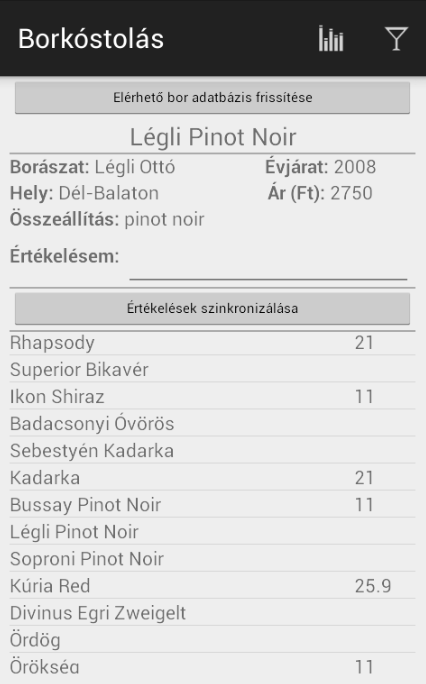
\includegraphics[scale=0.5]{UserPage}
		\caption[UserPage]{UserPage}
		\label{fig:UserPage}
	\end{figure}
	
	Az alsó $winesList$ részre ami egy $ListView$ -t tartalmaz és a bor adatbázis, valamint a felhasználó értékeléseinek megjelenítése a feladata, illetve a felső $detailsContainer$ részre amely $RelativeView$ -ot használ a $winesList$ -ban kiválasztott bor részletes adatainak megjelenítésére, valamint az értékeléshez szükséges bemeneti mező létrehozására. Az egész alkalmazás megalkotása során azt mondanám, hogy ennek a két résznek az összekötés, illetve kiszolgálása volt a legnehezebb feladat. Az egyik ilyen nehézség az volt, hogy a bemeneti mező alapértelmezetten előtérbe akar lenni az activity indításakor, ez pedig a virtuális billentyűzet előhívásával jár, ami kitakarta a $wineList$ nagy részét. Ezért a bemeneti mezőhöz használt $TextView$ elemre meg kellett hívnom a $setFocusable\left(\right)$ és a $setFocusableInTouchMode\left(\right)$ metódusokat $false$ paraméterrel. Egy másik felületi kezelhetőséggel kapcsolatos probléma a $winesList$ lista elemeinél jött elő, ugyanis nem lehetett rájuk kattintani, ezt a \ref{lst:ListView blocksDescendants} kódrészletben látott változó beállításával oldottam meg. Csak a fenti konfigurációs beállítások után sikerült elérni, hogy a felhasználói felület az elvártak szerint működjön, sajnos a két probléma kombinációja igen érdekes és számomra először nehezen értelmezhető tünetekkel került elő.
	
	\noindent\begin{minipage}{\linewidth}
		\begin{lstlisting}[language=java,label={lst:ListView blocksDescendants}, caption={A $ListView$ elmeinek előtérbehozhatóságnak beállítása}]
android:descendantFocusability="blocksDescendants" 
		\end{lstlisting}
	\end{minipage}
	
	\subsubsection{winesList}
	Ugyan a $ListView$ lista elemeihez van alapértelmezett elrendezés definiálva, ennek a kinézete nem illett a funkcióhoz. A bor neve és az értékelés egymás alá kerültek volna, ezért inkább definiáltam egy elrendezést saját magam a $winerow.xml$ állományban, amely lehetővé teszi azt, hogy akkor is olvasható legyen a borok neve, ha azok hossza meghaladná az adott mobil eszközön egy sorban elférő karakterek maximális szélességet. Ekkor a lista elem magassága úgy fog megnőni, hogy a szükséges sorok mind elférjenek. A bor neve, mellette jobb oldalon pedig a felhasználó által adott borra vonatkozó értékelés található, amely mindig vertikálisan középre van rendezve, így azon borok esetében is igényesen jelenik meg a pontszám, ha a nevük kiírásához több sorra lenne szükség. Súlyok használatával pedig azt értem el, hogy az értékelések ne csússzanak el a miatt, hogy a boroknak változó hosszúságú nevük van.
	
	A lista elemekkel való feltöltéséért a $WinesAdapter$ osztály felelős, amely az \linebreak$ArrayAdapter$ -ból származik és $ScoredWine$ típusú objektumokat kezel. A $getView\left(\right)$ metódus felüldefiniálására azért van szükség, mert nem az alapértelmezett lista elem elrendezést használtam. Az adott lista elem elrendezés adatokkal feltöltése a \ref{lst:ListView elem getView} kódrészletben látottak szerint történik.
	
	\noindent\begin{minipage}{\linewidth}
		\begin{lstlisting}[language=java,label={lst:ListView elem getView}, caption={Lista elem tartalmma való feltöltése}]
public View getView(int position, View convertView, ViewGroup parent) {
  ScoredWine wine = getItem(position);
  if (convertView == null) {
    convertView = LayoutInflater.from(getContext()).inflate(R.layout.winerow, parent, false);
  }   
  TextView tvName = (TextView) convertView.findViewById(R.id.wineRowName);
  TextView tvScore = (TextView) convertView.findViewById(R.id.wineRowScore);  
  tvName.setText(wine.getWine_name());
  Double score = wine.getWine_score();
  tvScore.setText(getFormattedScore(score));  
  return convertView;
}
		\end{lstlisting}
	\end{minipage}
	
	Látható, hogy a függvény első argumentumában kapott pozíció eleméhez tartozó \linebreak$ScoredWine$ objektumot az $ArrayList$ -ből a $getItem\left(\right)$ metódus másolja ki. A \linebreak$LayoutInflater$ példányosítja az egyedi lista elem elrendezést, amely elemeire így már hivatkozhatunk és adatokkal tölthetünk fel.
	
	Intuitívan ahhoz egy adott bort a felhasználó értékeljen, azt ki fogja választja a listából, de ahhoz, hogy a lista elemek gombként működjenek meg kell hívni a $wineList$ $setOnItemClickListener\left(\right)$ metódusát amely egy olyan $AdapterView$ \linebreak$OnItemClickListener\left(\right)$ vár amely legalább annak az $onItemClick\left(\right)$ metódusát felüldefiniálja. Ennek természetesen az egyik argumentuma a lista elem indexe, amely felhasználható az adatgyűjtésre a borokat tartalmazó $ArrayList$ -ből. Az így begyűjtött bor 
	objektum alapján fog feltöltődni a $detailsContainer$ tartalma. Egy talán kicsit sziszifuszi módon a bor objektum átadás az értékelő mező $setTag\left(\right)$ metódusán keresztül történik. Fontos, hogy itt kell engedélyezni azt is, hogy az értékeléseket fogadó bemeneti mező előtérbe kerülhessen, különben a felhasználó nem tudná majd értékelni a bort.
	
	\subsubsection{detailsContainer}
	Annak ellenére, hogy szerintem elég intuitív a felhasználói felület használata, mégis alapértelmezett esetben amikor az activity elindul ez az elrendezés üres és ahol a borok neve fog megjelenni az áll, hogy "Válasszon bort a listából". Miután a felhasználó kiválasztott egy értékelendő bort, annak attribútumai alapján kitöltődnek a $detailsContainer$ releváns szövegmezői. A $winesList$ értékeléssel való frissítésre a legátfogóbb megközelítésnek az tűnt, hogy akkor frissítem a $winesList$ -ben az adott bor értékelését, ha a bemeneti mező kikerül az előtérből, majd utána értesítem a $winesList$ adapterét, hogy frissítse a nézetet. 
	
	Még egy kisebb dolog megvalósítására térnék ki: Amikor a felhasználó befejezte a bemeneti mező használatát, akkor az eredményeket a virtuális billentyűzeten az enter gomb megnyomásával véglegesítheti ami elvégzi a virtuális billentyűzet elrejtését. Viszont ha a felhasználó nem használ virtuális billentyűzetet, mert mondjuk egy bluetooth billentyűzetet használ, akkor vannak olyan Android verziók, amelyeken az enter gomb megnyomása után nem tűnne el a virtuális billentyűzet. Ennek orvosolásáért felül kell definiálni a bemeneti mező $OnEditorActionListener$ -jét és saját magunknak lekezelni az enter gomb lenyomását.
	
	\subsection{Results}
	A $Results$ az algoritmusok futtatásáért felelős activity egy egyszerű $WebView$ amely a web alkalmazás egy ennek a feladatnak az ellátására létrehozott és optimalizált állományát tölti be. Ebből következik, hogy az eredmények megtekintésének feltétele aktív internet kapcsolat, valamint a mobil eszközön található értékelések előzőleges szinkronizációja. Ennek a megközelítésnek köszönhetően a web alkalmazással egységes eredmény reprezentálásra van lehetőség, ahogy az a \ref{fig:TabletResults} ábrán is látszik.
	\begin{figure}[!ht]
		\centering
		\includegraphics[scale=0.5]{TabletResults}
		\caption[Results activity egy fektetett tableten]{Results activity egy fektetett tableten}
		\label{fig:TabletResults}
	\end{figure}
	
	\chapter{A weboldal és a mobil alkalmazás összekötése}
	A weboldal és a mobil alkalmazás összekötése úgynevezett szolgáltatásokkal történik, amelyeket a web szerver tesz elérhetővé. Ezen szolgáltatások lényegébe véve PHP fájlok amelyek úgy lettek kialakítva, hogy első sorban a mobil alkalmazás által könnyen feldolgozható kimenetet produkáljak, ami konkrétan a legtöbb esetben egy az adatokat JSON string formátumban ábrázoló objektum.
	
	Mielőtt a mobil alkalmazás megpróbálja elérni ezeket a szolgáltatásokat, meg kell róla győződni, hogy az eszköz rendelkezik internet kapcsolattal. Ez már az előző fejezetben ismertetett $NetworkChecker$ osztály segítségével történik.
	
	A szolgáltatások kialakításánál során kicsi, lényegre törő kód írása volt a célom. A szolgáltatások csak az adatokat szolgáltatják, vagy a már előkészített csomagot töltik be a web szerver adatbázisba. A feldolgozást maga az Android alkalmazás végzi az alfejezetekben látható módon.
	
	Még mielőtt belemélyülnénk a szolgáltatások specifikus kezelésébe, mindenképpen érdemes néhány szót ejteni az Android alkalmazás szálkezeléséről. A fejlesztés során nagyon könnyű bele futni a $NetworkOnMainThreadException$ -be, amely akkor következik be, amikor az alkalmazás hálózati műveletet próbál végrehajtani a fő szálában. Annak ellenére, hogy ez csak az Android $Honeycomb$ verziója után lett bevezetve, mégis érdemes ezt elkerülnünk, feltéve, hogy az alkalmazásunk támogatja ezt az SDK verziót. Ezt könnyen elkerülhetjük, ha minden hálózati műveletet egy új szálon végzünk el, erre látható példa a \ref{lst:new thread for network} kódrészletben is.
	
	\noindent\begin{minipage}{\linewidth}
		\begin{lstlisting}[language=java,label={lst:new thread for network}, caption={Új szál létrehozásra}]
new Thread(new Runnable() {
  public void run() {
    // Halozati muvelet itt!
  }
}).start();
		\end{lstlisting}
	\end{minipage}
	
	Ennek a megszorításnak a betartása könnyen vezet a másik hibához, amely abból fakad, hogy a felhasználói felület elemeit próbáljuk manipulálni egy olyan szálból ami nem az alkalmazás fő szála. Ez pedig az activity-kben a  $runOnUiThread\left(\right)$ segítségével érhető el, amely a $Thread$ -nél látottakhoz hasonlóan egy $Runnable$ objektumot vár.
	
	\section{RemoteDAO}
	Az Android alkalmazás távoli adatbázis elérésért felelős osztálya amely az előző fejezetben látott $DAO$ interface metódusait implementálja. A $POST$ műveletek elvégzésért az $org.apache.http.client$ csomag felelős.
	
	\noindent\begin{minipage}{\linewidth}
		\begin{lstlisting}[language=java,label={lst:service access}, caption={Szolgáltatás használat példa}]
httpclient=new DefaultHttpClient();
httppost= new HttpPost("http://bor.tvarga.hu/services/getWineData.php"); // make sure the url is correct.
ResponseHandler<String> responseHandler = new BasicResponseHandler();
String result = httpclient.execute(httppost, responseHandler);
JSONArray jsonArray = new JSONArray(result);
for (int i=0; i < jsonArray.length(); i++ ){
  JSONObject obj = (JSONObject) jsonArray.get(i);
  Wine wine = JSONParser.getWineFromJSONObj(obj);
  wines.add(wine);
}
		\end{lstlisting}
	\end{minipage}
	
	A \ref{lst:service access} kódrészletben látott példa mutatja be, hogyan lehet a web alkalmazás egy szolgáltatását használni. A példa konkrétan az értékelhető borok adatbázisát tölti le. Jól látható, hogy ez egy paraméter nélküli URL használatával történik, de léteznek olyan szolgáltatások is, amelyek például a $user\_id$ -t továbbítják a kéréssel. Ilyenkor a változókat egy $BasicNameValuePair$ -ba kell tenni, amelyeket listába gyűjtve először bele kell formázni az URL-be a $UrlEncodedFormEntity\left(\right)$ segítségével, hogy aztán beállíthassuk $httpost$ entitását $setEntity\left(\right)$ -vel. Fontos, hogy a szolgáltatás által küldött válaszokat minden esetben fel kell dolgozni. 
	
	\section{Bejelentkezés}
	A $Main$ activity-n megadott belépési információkat a $RemoteDAO$ -nál már ismertetett módon küldjük el a web alkalmazásnak, amely szerver oldalon ellenőrzi, hogy azok helyesek voltak -e, be lehet -e léptetni ezekkel az információkkal a felhasználót. Mint már tárgyaltuk, biztonsági megfontolásokból, hibás adatok esetén csak egy generikus hiba üzenetet írunk ki, de ha sikeres volt a belépés, akkor a $Main Activity$ ismertetésénél látottak szerint lép tovább az Android alkalmazás.
	
	\section{Adatbázis szinkronizáció}
	Mivel a \ref{lst:service access} kódrészletben már láttunk példát az értékelhető borok letöltésére, most nézzük meg hogyan történik a felhasználó értékeléseinek szinkronizációja.
	
	Az első lépés az, hogy indítunk egy új szálat, hiszen hálózati műveleteket készülünk csinálni, amelyet egyből követhet is a hálózat meglétének ellenőrzése a már megszokott módon. Eddig nincs semmi újdonság.
	
	\subsection{syncScores}
	A $DBSyncController$ osztály $syncScores\left(\right)$ metódusa felelős az értékelések szinkronizációjáért. Itt az első lépés az adatbázis elérést biztosító osztályok példányosítása, majd azok respektív használatával az értékelés $ArrayList<Score>$ -ba való gyűjtése $remoteScores$, illetve $localScores$ változó nevek alatt.
	
	Amennyiben a $remoteScores$ tartalmazott értékeléseket azt átadjuk a $LocalDAO$ \linebreak$addOrUpdateScore\left(\right)$ -nak, amely feladata a lokális adatbázis frissítése. Ez úgy történik, hogy minden egyes $remoteScores$ értékelésére megnézzük, hogy a lokális adatbázisban van -e bejegyzés az adott $user\_id$ és $wine\_id$ kombinációval. Amennyiben igen, meg kell vizsgálni, hogy az értékelések megegyeznek -e, illetve, hogy a távoli értékelés nem -e volt korábban létrehozva mint a lokális, mert ha a két feltétel közül bármelyik teljesül, akkor nem kell frissíteni a lokális adatbázist. Viszont ha ezen feltételek nem teljesülnek, vagy nem volt még bejegyzés a lokális adatbázisban, akkor egyszerűen csak beszúrjuk azt. Ezzel be is fejeztük a helyi adatbázis frissítését.
	
	A következő feladat egy olyan JavaScript tömb létrehozása lesz amely első eleme a felhasználó neve, azt pedig a szinkronizált értékelések követik oly módon, hogy amennyiben a bor nem volt értékelve az a tömb elem üresen marad. Ezt a tömböt tovább adjuk a $RemoteDAO.addOrUpdateScore\left(()\right)$ metódusának, ahol máris láthatjuk miért volt szükség a JavaScript tömb használatára. A tömbre hívott $toString\left(\right)$ segítségével az adatok bele formázhatók az URL-be amely arra a szolgáltatásra mutat, ami a távoli adatbázisban való értékelések frissítéséért felelős. Itt kerül újra felhasználásra ugyan az az állomány amely a web alkalmazásban ugyan ezt a feladatot látta el.
	
	\subsection{Felhasználói felület frissítése}
	Még mielőtt rátérnénk az adatok reprezentálásának tényleges frissítésére, röviden megemlíteném, hogy a szinkronizációs folyamat során egy $Dialog$ ugrik fel, amely zárolja a felhasználói felületet a szinkronizáció befejeztéig. A sikerességéről vagy sikertelenségről pedig egy $Toast$ üzenetben értesítjük a felhasználót.
	
	Az értékelések sikeres szinkronizálása után nincs más dolgunk mint az Android alkalmazás felhasználói felületének frissítése. Amire oda kell figyelni az az, hogy ha \linebreak$detailsContainer$ éppen egy olyan bor adataival van feltöltve amelynek megváltozott a helyi adatbázisban az értékelése, akkor az input mezőben azt frissíteni kell. Valamint értesítenünk kell a $winesList$ -et arról, hogy az általa reprezentált adatsor megváltozott. Ezt végzi el a már korábban röviden említésre került $OnAdapterNeedsNotify$ interface egy implementált osztályának példánya esemény tüzelés segítségéve.
	
	\section{Eredmények}
	Az algoritmusok eredményének megjelenítése is tekinthető egy fajta szolgáltatásnak, amely a felhasználó azonosítója alapján generálja a megjelenítendő tartalmat az android alkalmazás számra. Nem tartozik ide szorosan, de érdekes lehet talán az, hogy az algoritmust választó legördülő menü használata magával vonja a számolások indítását. Ez a \ref{lst:dropdown onSelectChange} kódrészletben látott kódnak köszönhető.
	
	\noindent\begin{minipage}{\linewidth}
		\begin{lstlisting}[language=html,label={lst:dropdown onSelectChange}, caption={Legordülő menübeli algoritmus választás egyből indítja a számolást}]
<select id='algoritmus' name='Algoritmus' onchange='onSelectChange()' style="width: 100%;">
		\end{lstlisting}
	\end{minipage}
	
	
	\chapter{Tesztelés}
	Itt szeretném bemutatni az általam végzett néhány teszt esetet és azok eredményét, teszt procedúrákra bontva.
	
	\newcounter{TP}
	\setcounter{TP}{1}
	\newcounter{TC}
	\setcounter{TC}{1}
	\newcounter{TPTCStart}
	\newcounter{TPTCStop}
	
	\section{Regisztrációs és bejelentkeztető rendszer}
	
	% % % % % % % % % % % % % % % % % % % % % % % % % % % % % % % % % % % % % % % 
	
	\addtocontents{toc}{\protect\setcounter{tocdepth}{1}}
	\subsection{Tesztesetek}
	\addtocontents{toc}{\protect\setcounter{tocdepth}{2}}
	\setcounter{TPTCStart}{\value{TC}}
	
	\subsubsection{ID: TC\_\arabic{TC}}\addtocounter{TC}{1}
	\textbf{Teszteljárás:} TP\_\arabic{TP}
	\newline 
	\textbf{Leírás:} Regisztráció megfelelő adatok megadásával.
	\newline 
	\textbf{Bemenet:} $user\_name = "tom"$ $user\_password_new = "tom123"$ \linebreak$user\_password\_repeat = "tom123"$ $user\_email = "tom@tvarga.hu"$ $captcha = korrekt$
	\newline 
	\textbf{Action:} Az adatok beírása után a "Regisztráció" gombra kattintok.
	\newline 
	\textbf{Elvárt kimenet:} Hibaüzenet nélkül tér vissza.
	
	\subsubsection{ID: TC\_\arabic{TC}}\addtocounter{TC}{1}
	\textbf{Teszteljárás:} TP\_\arabic{TP}
	\newline 
	\textbf{Leírás:} Regisztráció nem megfelelő adatok megadásával.
	\newline 
	\textbf{Bemenet:} $user\_name = "t"$ $user\_password_new = "tom123"$ \linebreak$user\_password\_repeat = "tom123"$ $user\_email = "tom@tvarga.hu"$ $captcha = korrekt$
	\newline 
	\textbf{Action:} Az adatok beírása után a "Regisztráció" gombra kattintok.
	\newline 
	\textbf{Elvárt kimenet:} Hibaüzenettel tér vissza.
	
	\subsubsection{ID: TC\_\arabic{TC}}\addtocounter{TC}{1}
	\textbf{Teszteljárás:} TP\_\arabic{TP}
	\newline 
	\textbf{Leírás:} Regisztráció hiányos adat mezőkkel.
	\newline 
	\textbf{Bemenet:} $user\_name = ""$ $user\_password_new = "tom123"$ $user\_password\_repeat = "tom123"$ $user\_email = "tom@tvarga.hu"$ $captcha = korrekt$
	\newline 
	\textbf{Action:} Az adatok beírása után a "Regisztráció" gombra kattintok.
	\newline 
	\textbf{Elvárt kimenet:} Hibaüzenettel tér vissza.
	
	\subsubsection{ID: TC\_\arabic{TC}}\addtocounter{TC}{1}
	\textbf{Teszteljárás:} TP\_\arabic{TP}
	\newline 
	\textbf{Leírás:} Regisztráció hibás captcha megadásával.
	\newline 
	\textbf{Bemenet:} $user\_name = "tom1"$ $user\_password\_new = "tom123"$ \linebreak$user\_password\_repeat = "tom123"$ $user\_email = "tom@tvarga.hu"$ $captcha = hibás$
	\newline 
	\textbf{Action:} Az adatok beírása után a "Regisztráció" gombra kattintok.
	\newline 
	\textbf{Elvárt kimenet:} Hibaüzenettel tér vissza.
	
	\setcounter{TPTCStop}{\value{TC}}
	\addtocontents{toc}{\protect\setcounter{tocdepth}{1}}
	\subsection{Teszteljárás}
	\addtocontents{toc}{\protect\setcounter{tocdepth}{2}}
	\textbf{ID:} TP\_\arabic{TP}\addtocounter{TP}{1}
	\newline
	\textbf{Tesztesetek:} 
	\forloop{TPTCStart}{\value{TPTCStart}}{\value{TPTCStart} < \value{TPTCStop}}{
		TC\_\arabic{TPTCStart} 
	}
	\newline
	\textbf{Leírás:} Ez a teszteljárás a regisztráció tesztelésének lépéseit írja le.
	\newline
	\textbf{Lépések:}
	\begin{enumerate}
		\item Regisztrációs oldal betöltése.
		\item Felhasználónév, e-mail, jelszó, kapcsa megadása
		\item Regisztráció gomb megnyomása
		\item Visszajelzés értékelése 
	\end{enumerate}
	
	
	% % % % % % % % % % % % % % % % % % % % % % % % % % % % % % % % % % % % % % % 
	
	\addtocontents{toc}{\protect\setcounter{tocdepth}{1}}
	\subsection{Tesztesetek}
	\addtocontents{toc}{\protect\setcounter{tocdepth}{2}}
	\setcounter{TPTCStart}{\value{TC}}
	
	\subsubsection{ID: TC\_\arabic{TC}}\addtocounter{TC}{1}
	\textbf{Teszteljárás:} TP\_\arabic{TP}
	\newline 
	\textbf{Leírás:} Belépés megfelelő adatok megadásával.
	\newline 
	\textbf{Bemenet:} $user\_name = "tom"$ $user\_password = "tom123"$
	\newline 
	\textbf{Action:} Az adatok beírása után a "Bejelentkezés" gombra kattintok.
	\newline 
	\textbf{Elvárt kimenet:} Hibaüzenet nélkül tér vissza.
	
	\subsubsection{ID: TC\_\arabic{TC}}\addtocounter{TC}{1}
	\textbf{Teszteljárás:} TP\_\arabic{TP}
	\newline 
	\textbf{Leírás:} Belépés nem megfelelő adatok megadásával.
	\newline 
	\textbf{Bemenet:} $user\_name = "t"$ $user\_password = "tom123"$
	\newline 
	\textbf{Action:} Az adatok beírása után a "Bejelentkezés" gombra kattintok.
	\newline 
	\textbf{Elvárt kimenet:} Hibaüzenettel tér vissza.
	
	\subsubsection{ID: TC\_\arabic{TC}}\addtocounter{TC}{1}
	\textbf{Teszteljárás:} TP\_\arabic{TP}
	\newline 
	\textbf{Leírás:} Belépés megfelelő adatok megadásával.
	\newline 
	\textbf{Bemenet:} $user\_name = "tom"$ $user\_password = "tom123"$
	\newline 
	\textbf{Action:} Az adatok beírása után a "Bejelentkezés" gombra kattintok.
	\newline 
	\textbf{Elvárt kimenet:} Hibaüzenet nélkül tér vissza.
	
	\setcounter{TPTCStop}{\value{TC}}
	\addtocontents{toc}{\protect\setcounter{tocdepth}{1}}
	\subsection{Teszteljárás}
	\addtocontents{toc}{\protect\setcounter{tocdepth}{2}}
	
	\textbf{ID:}  TP\_\arabic{TP}\addtocounter{TP}{1}
	\newline
	\textbf{Tesztesetek:} 
	\forloop{TPTCStart}{\value{TPTCStart}}{\value{TPTCStart} < \value{TPTCStop}}{
		TC\_\arabic{TPTCStart}  
	}
	\newline
	\textbf{Leírás:} Ez a teszteljárás a bejelentkezés tesztelésének lépéseit írja le.
	\newline
	\textbf{Lépések:}
	\begin{enumerate}
		\item Felhasználónév, jelszó megadása
		\item Belépés gomb megnyomása
		\item Visszajelzés értékelése 
	\end{enumerate}
	
	
	% % % % % % % % % % % % % % % % % % % % % % % % % % % % % % % % % % % % % % % 
	
	
	\section{Demo adatkezelésének ellenőrzése}
	
	% % % % % % % % % % % % % % % % % % % % % % % % % % % % % % % % % % % % % % % 
	
	\addtocontents{toc}{\protect\setcounter{tocdepth}{1}}
	\subsection{Tesztesetek}
	\addtocontents{toc}{\protect\setcounter{tocdepth}{2}}
	\setcounter{TPTCStart}{\value{TC}}
	
	\subsubsection{ID: TC\_\arabic{TC}}\addtocounter{TC}{1}
	\textbf{Teszteljárás:} TP\_\arabic{TP}
	\newline 
	\textbf{Leírás:} Egy megfelelő bor értékelés megadás.
	\newline 
	\textbf{Bemenet:} $wine\_score\_1 = 15$
	\newline 
	\textbf{Action:} Az adatok beírása után az "Elküld" gombra kattintok.
	\newline 
	\textbf{Elvárt kimenet:} Hibaüzenet nélkül tér vissza.
	
	\subsubsection{ID: TC\_\arabic{TC}}\addtocounter{TC}{1}
	\textbf{Teszteljárás:} TP\_\arabic{TP}
	\newline 
	\textbf{Leírás:} Egy nem megfelelő bor értékelés megadás.
	\newline 
	\textbf{Bemenet:} $wine\_score\_1 = "a15"$
	\newline 
	\textbf{Action:} Az adatok beírása után az "Elküld" gombra kattintok.
	\newline 
	\textbf{Elvárt kimenet:} Hibaüzenettel tér vissza.
	
	\subsubsection{ID: TC\_\arabic{TC}}\addtocounter{TC}{1}
	\textbf{Teszteljárás:} TP\_\arabic{TP}
	\newline 
	\textbf{Leírás:} Több megfelelő bor értékelés megadás.
	\newline 
	\textbf{Bemenet:} $wine\_score\_1 = 15$ $wine\_score\_2 = 4$
	\newline 
	\textbf{Action:} Az adatok beírása után az "Elküld" gombra kattintok.
	\newline 
	\textbf{Elvárt kimenet:} Hibaüzenet nélkül tér vissza.
	
	\subsubsection{ID: TC\_\arabic{TC}}\addtocounter{TC}{1}
	\textbf{Teszteljárás:} TP\_\arabic{TP}
	\newline 
	\textbf{Leírás:} Több nem megfelelő bor értékelés megadás.
	\newline 
	\textbf{Bemenet:} $wine\_score\_1 = "a15"$ $wine\_score\_2 = "b4"$
	\newline 
	\textbf{Action:} Az adatok beírása után az "Elküld" gombra kattintok.
	\newline 
	\textbf{Elvárt kimenet:} Hibaüzenettel tér vissza.
	
	\subsubsection{ID: TC\_\arabic{TC}}\addtocounter{TC}{1}
	\textbf{Teszteljárás:} TP\_\arabic{TP}
	\newline 
	\textbf{Leírás:} Egy bor értékelésének törlése.
	\newline 
	\textbf{Bemenet:} $wine\_score\_1 = ""$
	\newline 
	\textbf{Action:} Az adatok beírása után az "Elküld" gombra kattintok.
	\newline 
	\textbf{Elvárt kimenet:} Hibaüzenet nélkül tér vissza.
	
	\subsubsection{ID: TC\_\arabic{TC}}\addtocounter{TC}{1}
	\textbf{Teszteljárás:} TP\_\arabic{TP}
	\newline 
	\textbf{Leírás:} Több bor értékelésének törlése.
	\newline 
	\textbf{Bemenet:} $wine\_score\_1 = ""$ $wine\_score\_2 = ""$
	\newline 
	\textbf{Action:} Az adatok beírása után az "Elküld" gombra kattintok.
	\newline 
	\textbf{Elvárt kimenet:} Hibaüzenet nélkül tér vissza.
	
	\setcounter{TPTCStop}{\value{TC}}
	\addtocontents{toc}{\protect\setcounter{tocdepth}{1}}
	\subsection{Teszteljárás}
	\addtocontents{toc}{\protect\setcounter{tocdepth}{2}}
	
	\textbf{ID:}  TP\_\arabic{TP}\addtocounter{TP}{1}
	\newline
	\textbf{Tesztesetek:} 
	\forloop{TPTCStart}{\value{TPTCStart}}{\value{TPTCStart} < \value{TPTCStop}}{
		TC\_\arabic{TPTCStart}  
	}
	\newline
	\textbf{Leírás:} Ez a teszteljárás $demo.php$ tesztelésének lépéseit írja le.
	\newline
	\textbf{Lépések:}
	\begin{enumerate}
		\item $demo.php$ betöltése
		\item Értékelés megadása
		\item Értékel gomb megnyomása
		\item Visszajelzés értékelése 
	\end{enumerate}
	
	
	% % % % % % % % % % % % % % % % % % % % % % % % % % % % % % % % % % % % % % % 
	
	\section{Adatbázis szinkronizáció}
	
	
	% % % % % % % % % % % % % % % % % % % % % % % % % % % % % % % % % % % % % % % 
	
	\addtocontents{toc}{\protect\setcounter{tocdepth}{1}}
	\subsection{Tesztesetek}
	\addtocontents{toc}{\protect\setcounter{tocdepth}{2}}
	\setcounter{TPTCStart}{\value{TC}}
	
	\subsubsection{ID: TC\_\arabic{TC}}\addtocounter{TC}{1}
	\textbf{Teszteljárás:} TP\_\arabic{TP}
	\newline 
	\textbf{Leírás:} Egy megfelelő bor értékelés megadás.
	\newline 
	\textbf{Bemenet:} Értékelésem = 15
	\newline 
	\textbf{Action:} Az adatok beírása után az "Értékelések szinkronizálása" gombra kattintok.
	\newline 
	\textbf{Elvárt kimenet:} Az értékelések helyesen szinkronizálódnak.
	
	\subsubsection{ID: TC\_\arabic{TC}}\addtocounter{TC}{1}
	\textbf{Teszteljárás:} TP\_\arabic{TP}
	\newline 
	\textbf{Leírás:} Több megfelelő bor értékelés megadás.
	\newline 
	\textbf{Bemenet:} Értékelésem1 = 15, Értékelésem2 = 4
	\newline 
	\textbf{Action:} Az adatok beírása után az "Értékelések szinkronizálása" gombra kattintok.
	\newline 
	\textbf{Elvárt kimenet:} Az értékelések helyesen szinkronizálódnak.
	
	\subsubsection{ID: TC\_\arabic{TC}}\addtocounter{TC}{1}
	\textbf{Teszteljárás:} TP\_\arabic{TP}
	\newline 
	\textbf{Leírás:} Egy megfelelő bor értékelés törlése.
	\newline 
	\textbf{Bemenet:} Értékelésem = ""
	\newline 
	\textbf{Action:} Az adatok beírása után az "Értékelések szinkronizálása" gombra kattintok.
	\newline 
	\textbf{Elvárt kimenet:} Az értékelések helyesen szinkronizálódnak.
	
	\subsubsection{ID: TC\_\arabic{TC}}\addtocounter{TC}{1}
	\textbf{Teszteljárás:} TP\_\arabic{TP}
	\newline 
	\textbf{Leírás:} Több megfelelő bor értékelés törlése.
	\newline 
	\textbf{Bemenet:} Értékelésem1 = "" Értékelésem2 = ""
	\newline 
	\textbf{Action:} Az adatok beírása után az "Értékelések szinkronizálása" gombra kattintok.
	\newline 
	\textbf{Elvárt kimenet:} Az értékelések helyesen szinkronizálódnak.
	
	
	\setcounter{TPTCStop}{\value{TC}}
	\addtocontents{toc}{\protect\setcounter{tocdepth}{1}}
	\subsection{Teszteljárás}
	\addtocontents{toc}{\protect\setcounter{tocdepth}{2}}
	
	\textbf{ID:}  TP\_\arabic{TP}\addtocounter{TP}{1}
	\newline
	\textbf{Tesztesetek:} 
	\forloop{TPTCStart}{\value{TPTCStart}}{\value{TPTCStart} < \value{TPTCStop}}{
		TC\_\arabic{TPTCStart}  
	}
	\newline
	\textbf{Leírás:} Ez a teszteljárás az adatbázis szinkronizáció tesztelésének lépéseit írja le.
	\newline
	\textbf{Lépések:}
	\begin{enumerate}
		\item Android alkalmazás elindítása
		\item Bejelentkezés
		\item Értékelés megadása
		\item Szinkronizáció gomb megnyomása
		\item Web alkalmazás $demo.php$ oldalának megnyitása
		\item Visszajelzés értékelése 
	\end{enumerate}
	
	
	% % % % % % % % % % % % % % % % % % % % % % % % % % % % % % % % % % % % % % % 
	
	\addtocontents{toc}{\protect\setcounter{tocdepth}{1}}
	\subsection{Tesztesetek}
	\addtocontents{toc}{\protect\setcounter{tocdepth}{2}}
	\setcounter{TPTCStart}{\value{TC}}
	
	\subsubsection{ID: TC\_\arabic{TC}}\addtocounter{TC}{1}
	\textbf{Teszteljárás:} TP\_\arabic{TP}
	\newline 
	\textbf{Leírás:} Egy megfelelő bor értékelés megadás.
	\newline 
	\textbf{Bemenet:} $wine\_score\_1 = 15$
	\newline 
	\textbf{Action:} Az adatok beírása után az "Elküld" gombra kattintok.
	\newline 
	\textbf{Elvárt kimenet:} Az értékelések helyesen szinkronizálódnak.
	
	\subsubsection{ID: TC\_\arabic{TC}}\addtocounter{TC}{1}
	\textbf{Teszteljárás:} TP\_\arabic{TP}
	\newline 
	\textbf{Leírás:} Több megfelelő bor értékelés megadás.
	\newline 
	\textbf{Bemenet:} $wine\_score\_1 = 15$, $wine\_score\_2 = 4$
	\newline 
	\textbf{Action:} Az adatok beírása után az "Elküld" gombra kattintok.
	\newline 
	\textbf{Elvárt kimenet:} Az értékelések helyesen szinkronizálódnak.
	
	\subsubsection{ID: TC\_\arabic{TC}}\addtocounter{TC}{1}
	\textbf{Teszteljárás:} TP\_\arabic{TP}
	\newline 
	\textbf{Leírás:} Egy megfelelő bor értékelés törlése.
	\newline 
	\textbf{Bemenet:} $wine\_score\_1 = ""$
	\newline 
	\textbf{Action:} Az adatok beírása után az "Elküld" gombra kattintok.
	\newline 
	\textbf{Elvárt kimenet:} Az értékelések helyesen szinkronizálódnak.
	
	\subsubsection{ID: TC\_\arabic{TC}}\addtocounter{TC}{1}
	\textbf{Teszteljárás:} TP\_\arabic{TP}
	\newline 
	\textbf{Leírás:} Több megfelelő bor értékelés törlése.
	\newline 
	\textbf{Bemenet:} $wine\_score\_1 = ""$, $wine\_score\_2 = ""$
	\newline 
	\textbf{Action:} Az adatok beírása után az "Elküld" gombra kattintok.
	\newline 
	\textbf{Elvárt kimenet:} Az értékelések helyesen szinkronizálódnak.
	
	
	\setcounter{TPTCStop}{\value{TC}}
	\addtocontents{toc}{\protect\setcounter{tocdepth}{1}}
	\subsection{Teszteljárás}
	\addtocontents{toc}{\protect\setcounter{tocdepth}{2}}
	
	\textbf{ID:}  TP\_\arabic{TP}\addtocounter{TP}{1}
	\newline
	\textbf{Tesztesetek:} 
	\forloop{TPTCStart}{\value{TPTCStart}}{\value{TPTCStart} < \value{TPTCStop}}{
		TC\_\arabic{TPTCStart}  
	}
	\newline
	\textbf{Leírás:} Ez a teszteljárás az adatbázis szinkronizáció tesztelésének lépéseit írja le.
	\newline
	\textbf{Lépések:}
	\begin{enumerate}
		\item Web alkalmazás $demo.php$ oldalának megnyitása
		\item Bejelentkezés
		\item Értékelés megadása
		\item Elküld gomb megnyomása
		\item Android alkalmazás elindítása
		\item Bejelentkezés
		\item Szinkronizáció gomb megnyomása
		\item Visszajelzés értékelése 
	\end{enumerate}
	
	\section{Algoritmusok ellenőrzése}
	A tesztelés ezen része még a weboldal egy korai verziója során történt meg, ezért az itt látható képek eltérhetnek a weboldal jelenlegi megjelenésétől.
	
	\subsection*{Kis adatokon}
	Az \ref{fig:algoritmus_kis_adatok} ábrán látható kis bemeneti adatokon akár kézzel is könnyen ellenőrizhető az implementált algoritmus működésének helyessége.
	\begin{figure}[!ht]
		\centering
		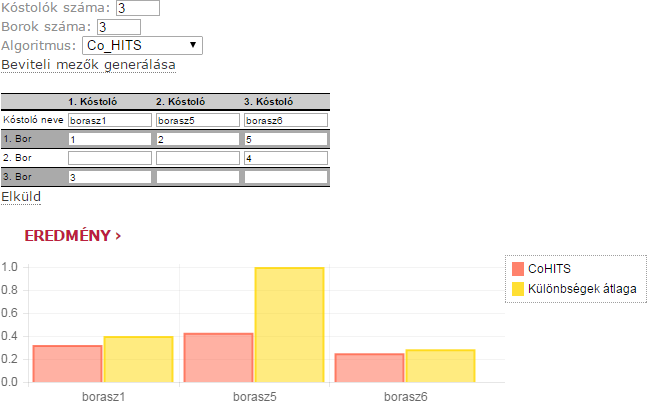
\includegraphics[width=0.7\linewidth]{algoritmus_kis_adatok}
		\caption[CoHITS kis adatokon futtatva]{CoHITS kis adatokon futtatva}
		\label{fig:algoritmus_kis_adatok}
	\end{figure}
	
	\subsection*{Ismert adatokon}
	Az algoritmus ellenőrzése a mellékletben található "júliusi vörös sorban.xls" alapján történt.
	
	\chapter{Egyebek}
	\section{Verziókezelés}
	
	\subsection*{Verziókezelés röviden}
	Ez alatt több verzióval rendelkező adatok kezelését értjük. Leggyakrabban a szoftverfejlesztésben használnak verziókezelő rendszereket fejlesztés alatt álló dokumentumok, tervek, forráskódok és egyéb olyan adatok verzióinak kezelésére, amelyeken több ember dolgozik egyidejűleg vagy amelyen több fizikai helyről dolgoznak.
	
	\subsection{Git}
	A \textbf{Git} egy nyílt forráskódú, elosztott verziókezelő szoftver, amely a sebességre helyezi a hangsúlyt amelyet eredetileg Linus Torvalds fejlesztette ki a Linux kernel fejlesztéséhez. Az elosztottság abban valósul meg, hogy a Git minden fejlesztő helyi munkaváltozatában rendelkezésre bocsátja a teljes addigi fejlesztési történetet, és a változtatások másolása mindig két repository között történik. Ezeket a változtatásokat mint külön ágakat importálják és összefésülhetőek, hasonlóan a helyben létrehozott fejlesztési ágakhoz. Ez azért jó, mert így minden munkamásolat egy teljes értékű repository teljes verziótörténettel és teljes revíziókövetési lehetőséggel, amely nem függ a hálózat elérésétől vagy központi szervertől.
	
	\subsection{GitHub}
	A GitHubot eredetileg Tom Preston-Werner, Chris Wanstrath és PJ Hyett hozta létre a kódmegosztási procedúra szimplifikálásának érdekében, mára a világ legnagyobb kód távoli kód repository szolgáltatójává nőtt \cite{Github}.
	
	\subsection{A választás} Már a kezdetektől nyilvánvaló volt számomra, hogy valamilyen verziókezelő rendszer használata elengedhetetlen lesz, mivel gyakran nem csak egy specifikus munkaállomásról szoktam dolgozni. Ez nem csak azért jó, mert nagyobb flexibilitást nyújt térben és időben, hanem azért is mert valamilyen szinten szimulálja azt amikor valaki egy projekt munkában egy közös kódbázison dolgozik. Korábbi munkáim és tanulmányaim során már néhány ilyen rendszerrel is megismerkedtem, többek között SVN, Git, Mercurial. A szakdolgozathoz tartozó alkalmazások készítéséhez végül a Git -et választottam mint verziókezelő rendszer, amelyhez távoli repository szolgáltatónak a GitHub társult. A választás fő támpontjai között talán a felhasználó barátságot és könnyű automatizálhatóságot említeném meg. 
	
	\subsection{Repozitóriumok}
	A szakdolgozat, web és android alkalmazás forráskódja az alábbi linkeken érhetők el:
	
	\begin{itemize}
		\item Szakdolgozat: \newline
		\url{https://github.com/TomVarga/borkostolas_szakdolgozat}
		\item Web alkalmazás: \newline \url{https://github.com/TomVarga/borkostolas_web_interface}
		\item Android alkalmazás: \newline \url{https://github.com/TomVarga/borkostolas_android_app}
	\end{itemize}
	
	
	\section{Környezetek}
	Itt szeretném bemutatni a fejlesztés során általam használt IDE (\textbf{I}ntegrated \textbf{D}evelopment \textbf{E}nvironment) és egyéb eszközöket és környezeteket. Valamint kitérnék a felhasználásuk során előkerült kisebb-nagyobb kellemetlenségekre vagy kedves meglepetésekbe.
	
	\subsection{SublimeText - linterek}
	A web alkalmazás fejlesztését a SublimieText 3 \cite{SublimeText} kód szerkesztővel kezdtem meg, mivel ezt használtam már több szkript nyelv alapú projekt realizálásához is. Ez a fejlesztői környezet jó néhány általam kedvelt szolgáltatással rendelkezik, csak, hogy néhányat említsek a sok közül:
	
	\begin{itemize}
		\item \textbf{Ugrás bárhová}: $Ctrl+P$ lenyomása után bármilyen már megnyitott fájlt könnyen fókuszba lehet hozni akár csak a nev egy részletének begépelésével, vagy ugyan itt lehet a $@$ használatával szimbólumhoz ugrani, $:$ -vel pedig egy adott sorra ugrani.
		\item \textbf{Command Palette}: $Ctrl+Shift+P$ segítségével sok időt meg lehet spórolni amely egyébként menü rendszerekben való keresgéléssel menne el. Egyszerűen csak elkezdjük begépelni a parancs egy részét amit végre szeretnénk hajtani és a lenyíló paletta automatikusan csak azokat a parancsokat fogja megjeleníteni amelyek tartalmazzák a már általunk begépelt részt.
		\item \textbf{Testre szabhatóság}: Szinte bármit személyre lehet szabni, legyen az: billentyű parancs, menük, jegyzetek, makrók, kód befejezés stb... Mind ehhez csak egy egyszerű JSON fájlt kell szerkeszteni amely lehetővé teszi, hogy az egyéni módosításaink csak fájl típusonként legyenek érvényesek vagy akár egész projektre vonatkozóan.
		\item \textbf{Többszörös kijelölés}: A többszörös kijelölésnek köszönhetően egyszerre tudunk elvégezni tíz módosítást ahelyett, hogy tízszer végeznének el ugyanazt az egy módosítást. Az oszlop kiválasztás is nagyon hatékonnyá teszi a kód rendezést, valamint a refaktorizációt, de persze itt említhetném meg az automatikus kód indentálást is.
		\item {Plugin API}: A Sublime Text rendelkezik egy nagy erejű Python alapú plugin API-val ami lehetővé teszi a környezet további kiváló szolgáltatásokkal való bővítését, mint például linterekkel vagy automatikus fájl feltöltő eszközökkel de itt említeném meg még a verziókezelőket támogató plugineket is.
	\end{itemize}
	
	A projekt automatikus FTP-re való feltöltéséhez a népszerű SFTP plugint használtam, amely ugyan úgy mint maga a Sublime Text egy $nagware$ termék (olyan shareware amely időnként általában egy előugró ablakkal arra kér minket, hogy vásároljuk licencet a termékhez). Ez gyorsan zavaróvá válhat, de egy egyszerű szkript segítségével könnyen elérhető, hogy az ilyen jellegű előugró ablakok automatikusan bezáródjanak.
	
	Bár a verzió kezelő rendszereket a Sublime Text alól mint parancssoros utasítások is lehet használni. Létezik konkrét Github Sublime Text plugin amely kényelmesebbé teheti az első beállításokat azok számára akik még nem jártasak a git verzió kezelő rendszer használatában. Én már korábbi projektekből rendelkeztem kisebb git szkriptekkel így a plugin nem igazán nyújtott olyan szolgáltatást amelyet korábban már ne implementáltam volna magamnak valamilyen formában.
	
	\paragraph{Linterek} Lintereknek nevezzük az olyan eszközöket amelyek gyanús kódhasználatra hívják fel a figyelmünket. A $lint$ eredetileg egy olyan program volt ami a $C$ forrás kódon ment végig gyanús, illetve valószínűleg bugos kódot keresve. Az ilyen jellegű eszközök általában statikusan vizsgálják a forrás kódot. Nagyon hasznosak tudnak lenni szintaktikai hibák felderítésében, vagy a modernebb változatok akár arra is fel tudják hívni a figyelmet, ha az adott kód nem felel meg egy adott kódolási stílus irányelvnek.
	
	\subsection{Android Studio}
	Az Android Studio \cite{Android Studio} az Android alkalmazásfejlesztőknek szánt hivatalos IDE amely a népszerű IntelliJ IDEA -n alapul. Az IntelliJ által elvárt szolgáltatásokon felül rendelkezik jó néhány Android specifikus és egyéb kiegészítéssel amelyek könnyebbé teszik a fejlesztés menetét:
	
	\begin{itemize}
		\item Gradle alapú buildelő rendszer
		\item Több fajta $apk$ fájl generálás
		\item Kód templatek és segítség népszerű alkalmazás szolgáltatások építéséhez
		\item Kibővített elrendezés szerkesztő, amely fogd meg és húzd alapú téma szerkesztés is lehetővé tesz
		\item Linter eszközök amelyek akár, teljesítmény, használhatóság vagy verzió kompatibilitási problémákra is fel tudják hívni a fejlesztő figyelmét
		\item ProGuard és alkalmazás aláíró képesség
		\item Támogatja a hordozható eszközöket is
		\item Beépített Google Clout Platform támogatás
	\end{itemize}
	
	A korábbi Eclipse alapú fejlesztő környezettel szemben itt már az SDK és Emulátor kezelő alkalmazások közvetlenül beépültek az IDE -be, egyszerűbbé téve azok menedzselését és telepítését.
	
	Mivel most először használtam ezt a fejlesztői környezetet, valamint Android fejlesztésben se voltam nagyon jártas ezért eltartott egy darabig mire rájöttem arra, hogy nem kell feltétlenül egy Nexus 5 alapú több gigabyte memóriával rendelkező emulátoron tesztelni az éppen fejlesztés alatt álló alkalmazást. Sokáig a Gradle build process akár egy két percet is igénybe vett. Mivel általában egy elég erős gépen fejlesztettem az Android alkalmazást ez egy idő után igen zavaróvá vált és jócskán hátráltatta a fejlesztés menetét. Csak miután rájöttem, hogy a régebbi Android verziók kisebb memória igénnyel rendelkeznek, valamint az emulátor snapshot használatának bekapcsolásával nagy mértékben sikerült felgyorsítani a build process-t így közvetetten a fejlesztés menetét is. Bár néhány nagyobb szolgáltatását mint például a keretrendszer támogatás még nem sikerült kipróbálnom. Könnyen el tudom képzelni, hogy a jövőben is ezt a fejlesztői környezetet fogom használni PHP projektet fejlesztéséhez.
	
	Bár az Android Studio is rendelkezik beépített verzió kezelő támogatással, első körben nem sikerült rávennem, hogy használja a szokásos módon megadott elérési úton lévő publikus kulcsomat. Csak kisebb kutakodás után sikerült kiderítenem, hogy ő azt egy konkrét helyen keresi és ha nem találja, akkor simán egy generikus hiba üzenettel fog visszatérni, amely szerint nem sikerült a távoli repozitóriumhoz csatlakozni, annak ellenére, hogy az nyílt és publikus is.
	
	\subsection{PhpStorm}
	A PhpStorm a JetBRAINS által fejlesztett PHP IDE amely harminc napig ingyenesen kipróbálható. A fő ok amiért kipróbáltam az volt, hogy már megszoktam az Android Studio nagyon intelligens kód kiegészítő szolgáltatását. Amikor vissza mentem a web alkalmazást csinosítgatni kicsit megterhelő volt a régi eszköz használata ezért elkezdtem keresni hátha létezik valamilyen IntelliJ alapú IDE amely támogatja PHP és a JavaScript nyelveket. Nagyon gyorsan sikerült is rátalálnom a PhpStorm -ra, amely teljes mértékben azt hozta amit vártam.
	
	Mivel a PhPStorm -ot csak az Android Studio megismerése után kezdtem el használni ezért különösebben nem találkoztam olyan dologgal benne ami nagy újdonság lett volna. A mentés utáni automatikus feltöltés beállítása könnyen ment elsőre is és pontosan az elvárt hierarchia szerint működött. Talán az egyetlen kisebb kényelmetlenség amely említésre méltó a fejlesztői környezet használata során a refaktorizáció használata. Lehetséges, hogy valahol be lehet állítani, hogy konstans stringebe is végezze el a refaktorizációt, de ezt az opciót nem találtam meg ezért kénytelen voltam mindig minden refaktorizáció után egy manuális projekt keretű keresést lefuttatni a már átnevezett vagy átmozgatott értékre, így meg tudtam győződni róla, hogy valóban minden példány ténylegesen átneveződött.
	
	\chapter{Összefoglalás}
	A szakdolgozat készítése során sikerült egy olyan web és mobil alkalmazást létrehoznom, amely egy könnyen kezelhető, letisztult, intuitívan használható, felhasználóbarát felületen keresztül mutatja ba néhány rangsoroló algoritmus működését borkóstolási értékelések alapján. A más projektből származó algoritmusok felhasználása és kisebb javítása hozzásegített ahhoz, hogy a további feladataim közé tartozó $CoHITS$ algoritmus implementálását véghezvigyem, amely mint kiderült jobban kezeli a hiányos bemeneti adatokat mint néhány alap statisztikai algoritmus. A web alkalmazás fejlesztése során lehetőségem nyílt népszerű modern technológiák és programozási nyelvek használatára, amelyek használatának köszönhetően könnyen találtam olyan nyílt könyvtár csomagokat amelyek az alkalmazás egyes kritikusabb részeinek kiszolgálására voltak alkalmasak.
	
	Az Android alkalmazás megtervezése és implementálása nagyon jó alkalmat nyújtott a tanult $MVC$ tervezési minta alkalmazására, valamint magára a mobil fejlesztés menetének megismerésére. A web és mobil alkalmazás összekötése jó példa arra, hogy miképp lehet egy web alkalmazás szolgáltatását elérhetővé tenni egy natív mobil felületen. Bár azt nem mondhatom, hogy az így elkészült első alkalmazásom teljes mértékben vetekszik a napjaink népszerű egyedi grafikával rendelkező erősen animált alkalmazásokkal. Mégis, a fejlesztés során szerzett tapasztalat mindenképpen egy jó alapot adott a jövőbeli továbbfejlődéshez. 
	
	%\begin{tét}
	%\label{tét-alap}
	%Ez itt egy tétel.
	%\end{tét}
	
	%%A bizonyítás \begin{proof} és \end{proof} közé kerül:
	%\begin{proof}
	%Ez pedig a bizonyítása, amelyben szerepel egy képlet:
	%\begin{equation}
	%\begin{split}
	%E^{\text{globális}} &= \text{tét}_1\cdot E_1^{\text{elemi}}+\text{tét}_2\cdot
	%E_2^{\text{elemi}}+\ldots+\text{tét}_n\cdot E_n^{elemi} \\
	%&=E^{\text{elemi}}\left(\text{tét}_1+\text{tét}_2+\ldots+\text{tét}_n\right)\\
	%&=E^{\text{elemi}}\cdot\text{össztét}
	%\end{split}
	%\end{equation}
	%A második egyenlőségnél azt használtunk ki, hogy ...
	%
	%Ezzel a bizonyítást befejeztük.
	%\end{proof}
	
	%\begin{defi}
	%\label{def-pelda}
	%Ez egy definíció. Számozása a tételekkel együtt történik.
	%\end{defi}
	
	%\begin{áll}
	%A követekező négy állítás egymással ekvivalens:
	%\label{áll-ekvivalencia}
	%  \begin{itemize}
	%  \item[(i)] $M$ és $N$ gyengén ekvivalensek.
	%  \item[(ii)] Minden $n$
	%  nemnegatív egész számra $|L_{M}\cap \Sigma_{1}^{n}|=|L_{N}\cap \Sigma_{2}^{n}|$ teljesül.
	%  \item[(iii)] Minden $n$ nemnegatív egész szám esetén
	%   létezik
	%  $ \pi_{n}: L_{M}\cap \Sigma_{1}^{n} \rightarrow L_{N}\cap \Sigma_{2}^{n} $ kölcsönösen egyértelmű
	%  leképezés.
	%  \item[(iv)] Minden nemnegatív $n$-re $x A^{n} y^{T}=x' A'^{n} y'^{T}$.
	%  \end{itemize}
	%\end{áll}
	
	%\begin{köv}
	%  Ez pedig egy következmény.
	%\end{köv}
	
	%\begin{pld}
	%  Ez lesz a példa, ezt nem szedjük dőlten.
	%\end{pld}
	
	%\begin{megj}
	%  A fejezetet pedig egy megjegyzés zárja.
	%\end{megj}
	
	%\section{Listák}
	%
	%Ez egy felsorolás:
	%\begin{itemize}
	%    \item első
	%    \item második
	%      \subitem első
	%      \subitem második
	%    \item harmadik
	%    \item[$\clubsuit$]  saját jel is alkalmazható
	%\end{itemize}
	%Ez pedig egy számozott lista:
	%\begin{enumerate}
	%            \item hétfő
	%            \item kedd
	%            \item szerda
	%\end{enumerate}
	
	%Oldaltörést is alkalmazhatunk
	\pagebreak
	
	
	%\section{Egy táblázat és egy ábra}
	%
	%A táblázat itt következik.
	%\begin{table}[!h]\label{strategia}
	%\caption{Példa stratégiatáblára a Black Jack esetében}
	%\begin{center}
	%\begin{tabular}{l||r|r|r|r|r|r|r|r|r|r}
	%&ász&2&3&4&5&6&7&8&9&10\\
	%\hline\hline
	%21&n&n&n&n&n&n&n&n&n&n\\
	%20&n&n&n&n&n&n&n&n&n&n\\
	%19&n&n&n&n&n&n&n&n&n&n\\
	%18&n&n&n&n&n&n&n&n&n&n\\
	%17&n&n&n&n&n&n&n&n&n&n\\
	%16&h&n&n&n&n&n&h&h&b&b\\
	%15&h&n&n&n&n&n&h&h&h&b\\
	%14&h&n&n&n&n&n&h&h&h&b\\
	%13&h&n&n&n&n&n&h&h&h&h\\
	%12&h&n&n&n&n&n&h&h&h&h\\
	%11&h&D&D&D&D&D&D&D&D&h\\
	%\end{tabular}
	%\end{center}
	%\end{table}
	%
	% % %%Lássunk egy ábrát is!
	%\begin{figure}[!h]
	%\unitlength 8mm
	%\begin{center}
	%\begin{picture}(8,6)
	%\thicklines
	%\multiput(0,1)(0,1){2}{\line(1,0){5}}
	%\multiput(3,0)(1,0){2}{\line(0,1){6}}
	%\multiput(1,0)(1,0){2}{\line(0,1){1}}
	%\multiput(6,0)(1,0){2}{\line(0,1){5}}
	%\multiput(0,1)(1,0){3}{\line(0,1){1}}
	%\multiput(2,4)(3,0){3}{\line(0,1){1}}
	%\multiput(3,0)(0,3){3}{\line(1,0){1}}
	%\multiput(6,0)(0,1){4}{\line(1,0){1}}
	%\multiput(7,2)(0,1){2}{\line(1,0){1}}
	%\multiput(2,4)(0,1){2}{\line(1,0){6}}
	%\put(5,1){\line(0,1){1}}
	%\put(8,2){\line(0,1){1}}
	%\put(1,0){\line(1,0){1}}
	%\put(1,1){\makebox(1,1){\(\sphericalangle\)}}
	%\put(7,2){\makebox(1,1){\(\$\)}}
	%\end{picture}
	%\end{center}
	%\caption{\label{labirintus}Labirintus bejárása}
	%\end{figure}
	
	%laptörés:
	%\newpage
	%
	%Külön fájlban elkészített grafika beillesztését a 
	%\ref{abra-automata} ábra szemlélteti.
	%\begin{figure}[h]
	%\centering
	%%A psfrag csomag használatával a (encapsulated)postcript abra feliratait LaTeX koddal helyettesíthatjük:
	%\psfrag{a}[c][c]{$q_0$}
	%\psfrag{b}[c][c]{$q_1$}
	%\psfrag{c}[c][c]{$q_2$}
	%\psfrag{d}[c][c]{$q_3$}
	%\psfrag{e}[c][c]{$q_4$}
	%\psfrag{f}[c][c]{$q_5$}
	%\psfrag{g}[c][c]{$q_6$}
	%\psfrag{h}[c][c]{$q_7$}
	%\psfrag{0}[c][c]{$a_{0}$}
	%\psfrag{9}[c][c]{$a_{9}$}
	%\psfrag{3}[c][c]{$a_{3}$}
	%\psfrag{12}[c][c]{$a_{12}$}
	%\psfrag{15}[c][c]{$a_{15}$}
	%%Garfika belillesztese, "scale2 a nagyitas/kicinyites merteke, itt 80%.
	%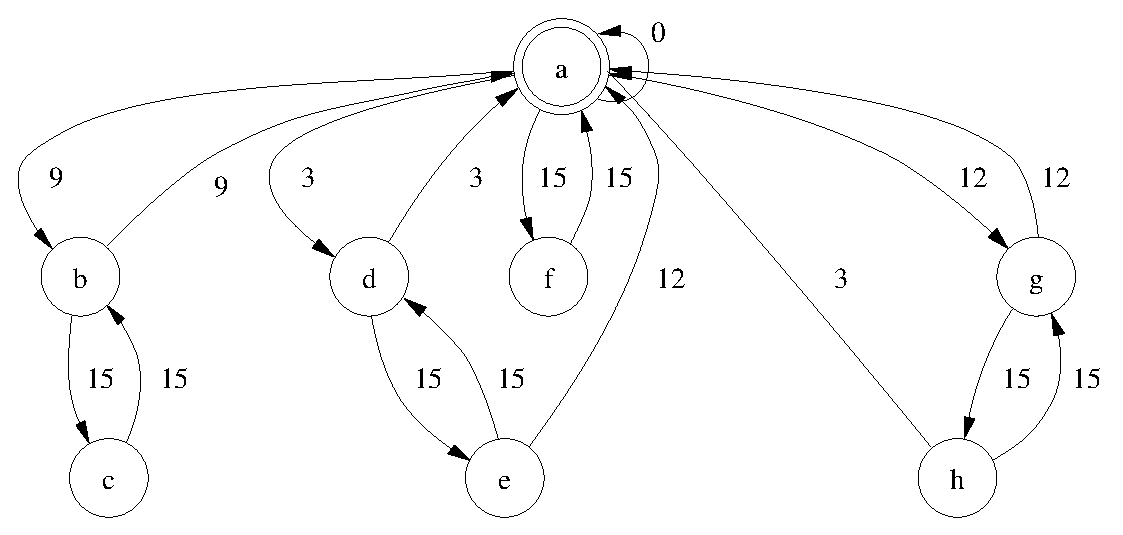
\includegraphics[scale=0.8]{abra.eps}
	%\caption{\label{abra-automata} A $4\times m$-es tábla lefedéseinek mátrixreprezentációit felismerő automata}
	%\end{figure}
	
	
	%\chapter{Függelék}
	%
	%\section{A program forráskódja}
	%A függelékbe kerülhetnek a hosszú táblázatok, vagy mondjuk egy programlista:
	%% A verbatim kornyezet hasznalatanal ügyeljünk rá, hogy az editor a szóközöjket át ne írja tab karakterekre!
	%\begin{verbatim}
	%   while (ujkmodosito[i]<0)
	%   {
	%      if (ujkmodosito[i]+kegyenletes[i]<0)
	%      {
	%         j=i+1;
	%         while (j<14)
	%         if (kegyenletes[i]+ujkmodosito[j]>-1) break;
	%         else j++;
	%         temp=ujkmodosito[j];
	%         for (l=i;l<j;l++) ujkmodosito[l+1]=ujkmodosito[l];
	%         ujkmodosito[i]=temp;
	%      }
	%      i++;
	%   }
	%\end{verbatim}
	
	
	
	\chapter*{Nyilatkozat}
	%Egy üres sort adunk a tartalomjegyzékhez:
	\addtocontents{toc}{\ }
	\addcontentsline{toc}{section}{Nyilatkozat}
	%\hspace{\parindent}
	
	% A nyilatkozat szövege más titkos és nem titkos dolgozatok esetében.
	% Csak az egyik tipusú myilatokzatnak kell a dolgozatban szerepelni
	% A ponok helyére az adatok értelemszerűen behelyettesídendők es
	% a szakdolgozat /diplomamunka szo megfeleloen kivalasztando.
	
	
	%A nyilatkozat szövege TITKOSNAK NEM MINŐSÍTETT dolgozatban a következő:
	%A pontokkal jelölt szövegrészek értelemszerűen a szövegszerkesztőben és
	%nem kézzel helyettesítendők:
	
	\noindent
	Alulírott Varga Tamás programtervező informatikus BSc szakos hallgató, kijelentem, hogy a dolgozatomat a Szegedi Tudományegyetem, Informatikai Tanszékcsoport Számítógépes Optimalizálás Tanszékén készítettem, programtervező informatikus BSc diploma megszerzése érdekében.
	
	Kijelentem, hogy a dolgozatot más szakon korábban nem védtem meg, saját munkám eredménye, és csak a hivatkozott forrásokat (szakirodalom, eszközök, stb.) használtam fel.
	
	Tudomásul veszem, hogy szakdolgozatomat a Szegedi Tudományegyetem Informatikai Tanszékcsoport könyvtárában, a helyben olvasható könyvek között helyezik el.
	
	\vspace*{2cm}
	
	\begin{tabular}{lc}
		Szeged, \today\
		\hspace{2cm} & \makebox[6cm]{\dotfill} \\
		& aláírás \\
	\end{tabular}
	
	
	
	\vspace*{4cm}
	
	
	
	%% Az itrodalomjegyzek keszitheto a BibTeX segedprogrammal:
	%\bibliography{diploma}
	%\bibliographystyle{plain}
	
	%VAGY "kézzel" a következő módon:
	
	\begin{thebibliography}{99}
		%10-nél kevesebb hivatkozás esetén
		\bibitem{Borkostolas projekt}Borkóstolás projekt.  \url{http://www.inf.u-szeged.hu/~tnemeth/osa/}
		
		\bibitem{PageRank}
		Sergey Brin and Lawrence Page. 
		The anatomy of a large-scale hypertextual web search engine. 
		\emph{ Computer Networks and ISDN Systems},
		\textbf{30}(1998), no 1, 107-117.
		
		\bibitem{HITS}
		J. Kleinberg. Authoritative sources in a hyperlinked environment.
		\emph{Journal of the ACM}, \textbf{46}(1999), no. 5, 604-632.
		
		\bibitem{Github}
		GitHub - \url{https://github.com/about}
		
		\bibitem{CoHITS}
		London András és Csendes Tibor. 
		HITS based network algorithm for evaluating the professional skills of wine tasters
		
		\bibitem{php-login}
		Panique. \url{http://www.php-login.net}
		
		\bibitem{php-history}
		History of PHP. \url{http://php.net/manual/en/history.php.php}
		
		\bibitem{CSS-origin}
		Lie, Hakon W (10 Oct 1994). Cascading HTML style sheets - a proposal
		
		\bibitem{PDO-charset-security}
		\url{http://wiki.hashphp.org/PDO\_Tutorial\_for\_MySQL\_Developers\#Connecting\_to\_MySQL}
		
		\bibitem{Google Charts homepage}
		Google Charts homepage
		\url{https://google-developers.appspot.com/chart/}
		
		\bibitem{Charts.js homepage}
		Charts.js homepage
		\url{http://www.chartjs.org/}
		
		\bibitem{ECMAScript Language Overview}
		ECMAScript Language Overview. 2007-10-23. p. 4. \url{http://www.ecmascript.org/es4/spec/overview.pdf}
		
		\bibitem{ECMAScript 5.1 release}
		ECMAScript Language Specification \url{http://www.ecma-international.org/publications/files/ECMA-ST/Ecma-262.pdf}
		
		\bibitem{deep linking for ajax}
		\url{http://blog.onthewings.net/2009/04/08/deep-linking-for-ajax/}
		
		\bibitem{numericjs source}
		Sébastien Loisel.
		Numeric Javascript. 
		\url{http://www.numericjs.com/}
		
		\bibitem{Gravatar}
		Gravatar.
		\url{http://www.gravatar.com/}
		
		\bibitem{SublimeText}
		SublimeText.
		\url{http://www.sublimetext.com/}
		
		\bibitem{Android Studio}
		Android Studio.
		\url{http://developer.android.com/tools/studio/index.html}
		
		%\begin{thebibliography}{99}
		% 10-nél több hivatkozás esetén
		
		\addcontentsline{toc}{section}{Irodalomjegyzék}
		
		%Elso szerzok vezetekneve alapjan ábécérendben rendezve.
		
		
		%folyóirat cikk: szerzok(k), a folyóirat neve kiemelve,
		%az evfolyam felkoveren, zarojelben az evszam, vegul az oldalszamok es pont.
		
		%\bibitem{Gischer}
		%J. L. Gischer,
		%The equational theory of pomsets.
		%\emph{Theoret. Comput. Sci.}, \textbf{61}(1988), 199--224.
		
		%könyv (szerzo(k), a könyv neve kiemelve, utana a kiado, a kiado szekhelye, az evszam es pont.)
		
		%\bibitem{Pin}
		%J.-E. Pin,
		%\emph{Varieties of Formal Languages},
		%Plenum Publishing Corp., New York, 1986.
		
		
	\end{thebibliography}
	
	
\end{document}
